\chapter{Search for Standard Model $\PH \to \Pgt\Pgt$}
\label{chap:httSM}

As described in chapter \ref{chap:theory}, the Higgs boson is the final missing 
piece of the Standard Model of particle physics. In order to complete the
\ac{SM}, this Higgs boson should have all the predicted properties of the
\ac{SM} Higgs, including decaying to tau leptons at the predicted rate. This
chapter describes the search for the Higgs boson of the Standard Model 
decaying into two tau leptons.

This chapter outlines the "legacy" result from run 1 of the \ac{LHC}, including the
full dataset collected in 2011 and 2012 by CMS. This corresponds to an
integrated luminosity of 4.9 fb$^{-1}$ at a centre of mass energy of 7 TeV and
19.7 fb$^{-1}$ at 8 TeV. The results in this chapter are parts of a publication 
in the Journal of High Energy Physics \cite{HIG-13-004}. The material included 
in this chapter is particularly focussed towards the parts of the analysis which 
included the work of the author. 

The $\PH \to \Pgt\Pgt$ analysis is performed in different final states dependent
on the final decay products of the taus. Taus can decay into electrons $e$,
muons $\mu$ and hadrons (denoted $\tau_{h}$), all with associated neutrinos.
This gives a total of six possible final states, $\ee$, $\mumu$, $\emu$,
$\etau$, $\mutau$ and $\tautau$. The most direct involvement of the author in this
analysis and the analyses in the subsequent chapters was for the $\etau$ and
$\mutau$ channels, although considerable work was also done on the statistical
interpretation side using results from all channels. 
As such the analysis details described in sections \ref{sec:eventSelection},
\ref{sec:backgrounds}, \ref{sec:datamcfactors} and \ref{} are focussed on the
$\etau$ and $\mutau$ channels, whilst results including the combination of all
six channels are shown in \ref{sec:results}. More detail on the other channels
can be found in \cite{HIG-13-004}. 

\section{Event Selection}
\label{sec:eventSelection}

This section describes how the objects described in chapter
\ref{chap:reco} are used to select the most signal-like events. 
The following sections describe in more detail the selections
used for each of the $\mutau$ and $\etau$ channels.

\subsection{Candidate Pair in the $\etau$ Channel}

Events in the $\etau$ channel are selected requiring an electron and hadronic tau
candidate. The electron is required to have $\pt$ larger than ($20~\GeV$)
$24~\GeV$ in (2011) 2012 data. In all data taking periods the $\eta$ requirement
on the electron is $|\eta| < 2.1$. The electron is required to pass the electron
ID \ac{BDT} as described in section \ref{sec:electrons}, using a $\pt$ and
$\eta$ dependent cut which corresponds to the tight working point.  
The isolation definition described in section \ref{sec:leptonisolation} is
applied with a threshold of 0.1. The electron must be compatible with
originating at the chosen \ac{PV}, and so the impact parameters in the
transverse and beam directions, $d_{xy}$ and $d_{z}$ respectively, must be
small. 

The hadronic tau is selected with $\pt$ of larger than $30~\GeV$ and
$|\eta|<2.3$. The tau is identified using the \ac{HPS} algorithm as described in 
section \ref{sec:hps}. The tau must be compatible with
originating at the chosen \ac{PV}, and so the impact parameters in the
transverse and beam directions, $d_{xy}$ and $d_{z}$ respectively, must be
small. As described in section \ref{sec:tauleptonrejection}, tau candidates are
required to pass criteria to reduce the mis-identification of electrons and
muons. In the $\etau$ channel, a tight working point for electron rejection is
used, and a loose working point for muon rejection. Isolation as described in
section \ref{sec:tauisolation} is applied is an optimised working point.  

The electron and hadronic tau are required to be of opposite charge. 
The $\pt$ and $\eta$ distributions of the candidate pair in the
$\etau$ channel are shown in figure \ref{fig:etauelectrons} for the electron and
\ref{fig:etautaus} for the tau. 


\begin{figure}[htb]
\begin{center}
\subfloat[]{
    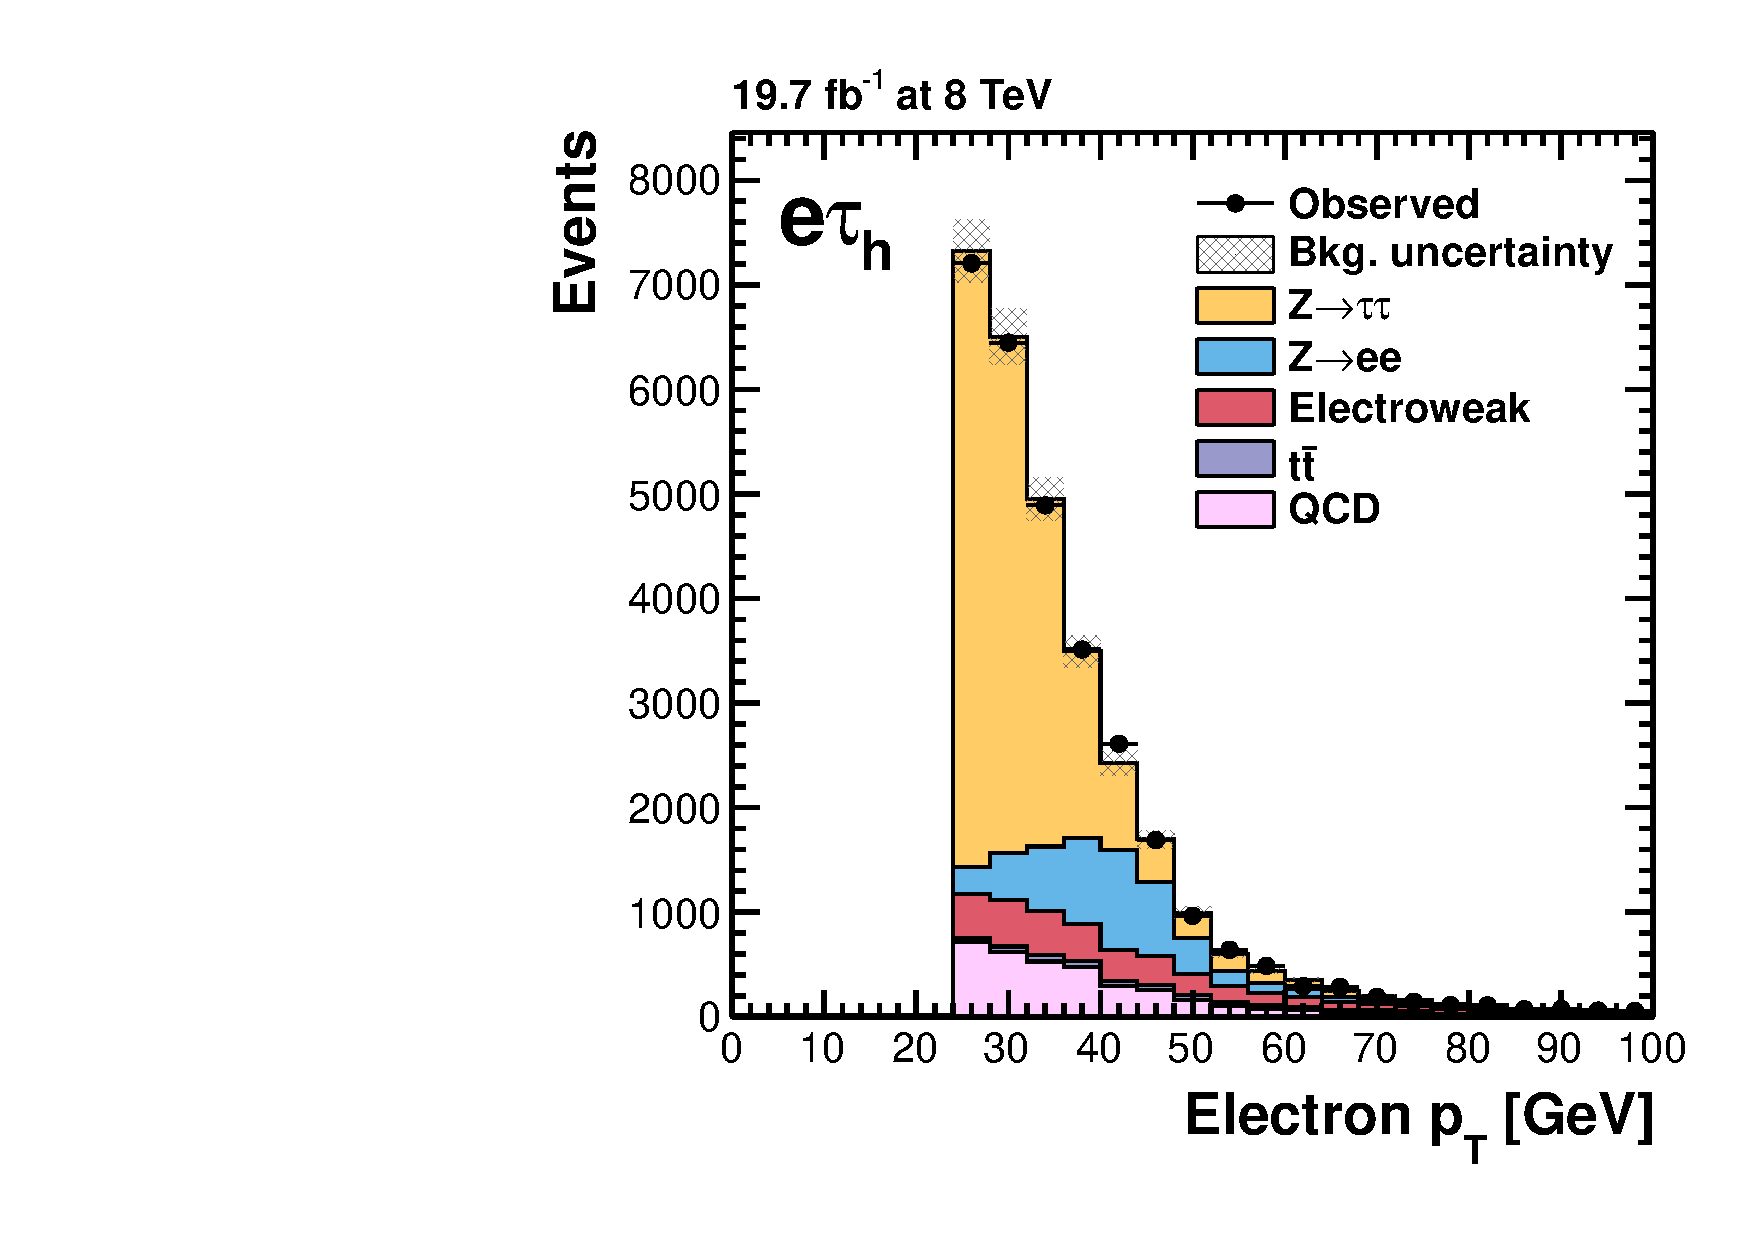
\includegraphics[width=0.5\textwidth]
      {plots/htt-sm/pt_1_inclusive_et_2012.pdf}}
\subfloat[]{
    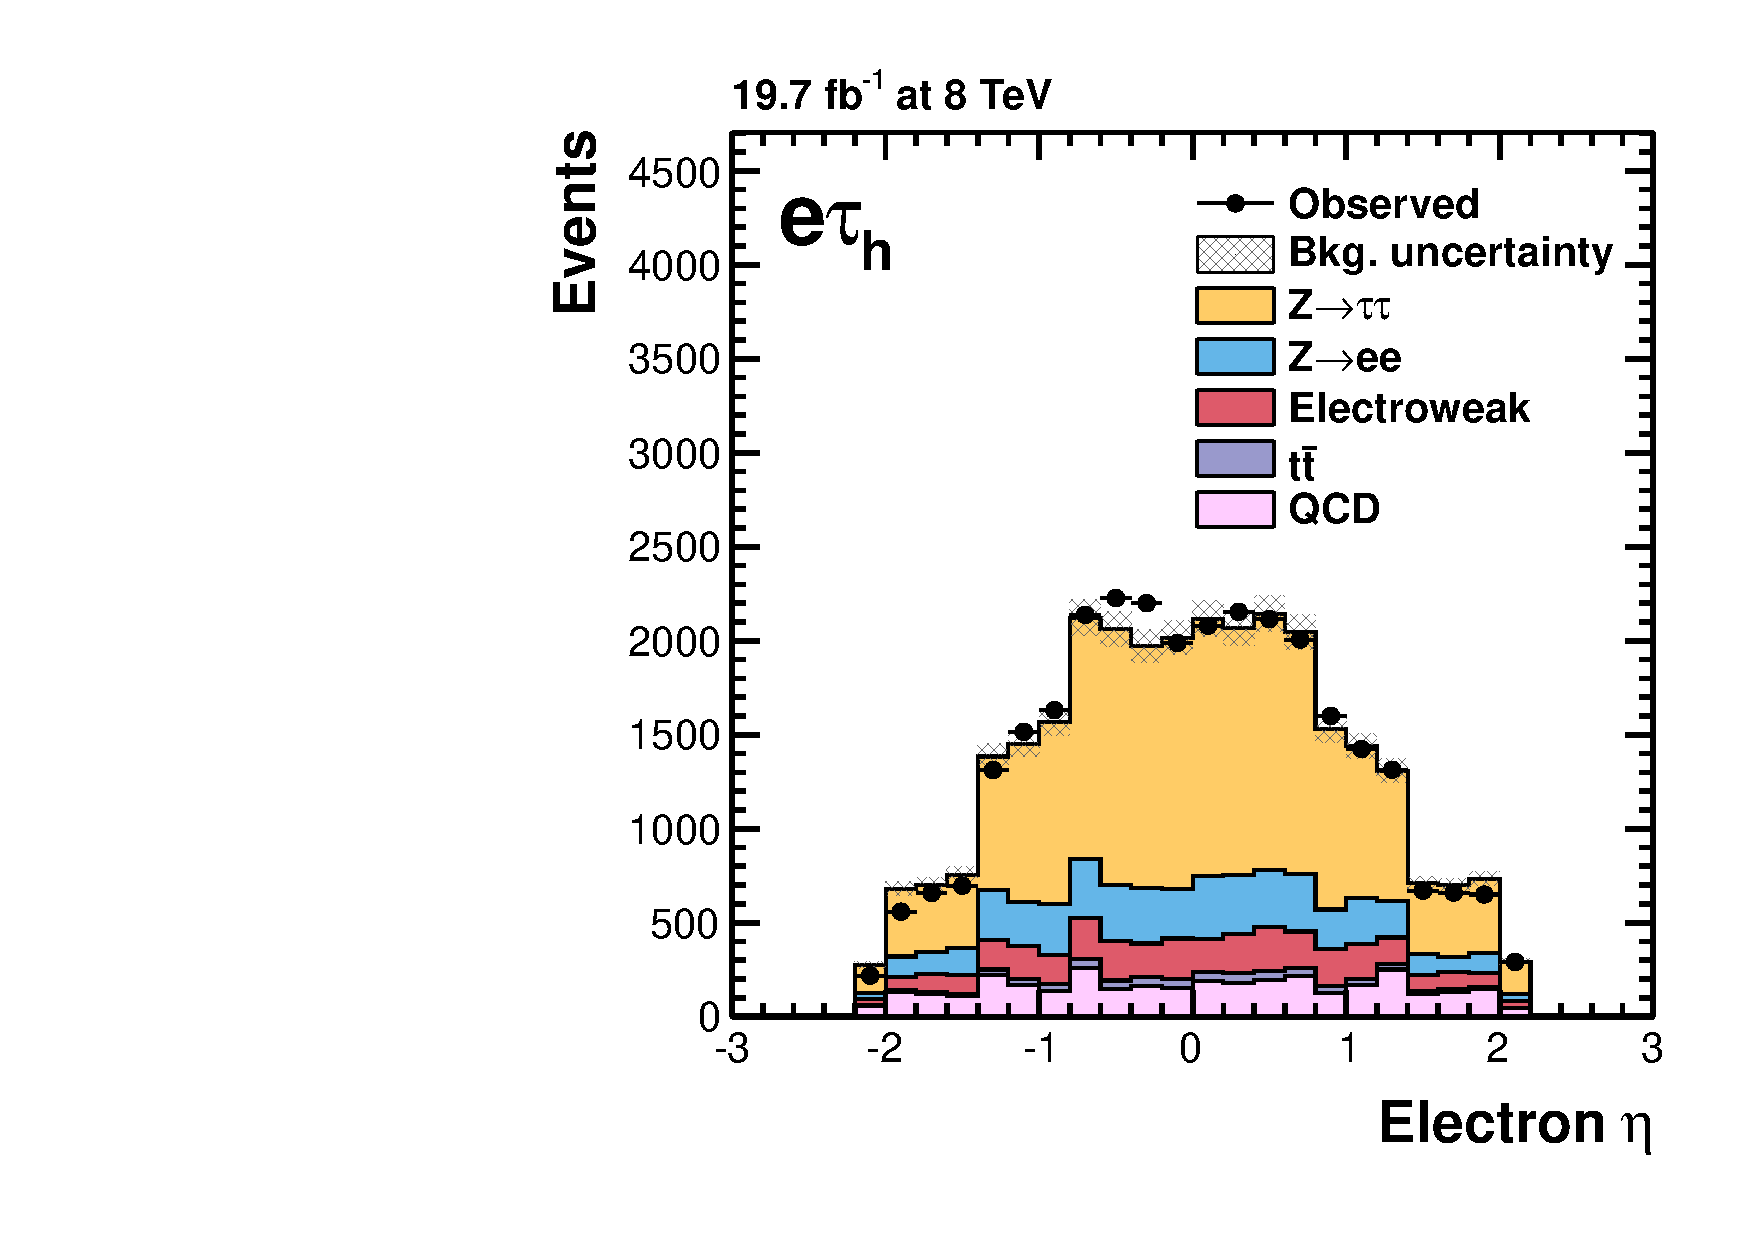
\includegraphics[width=0.5\textwidth] 
      {plots/htt-sm/eta_1_inclusive_et_2012.pdf}} 

\end{center}
\caption{
The $\pt$ and $\eta$ distribution for electron candidates in the $\etau$
channel.
}
\label{fig:etauelectrons}
\end{figure}


\begin{figure}[htb]
\begin{center}
\subfloat[]{
    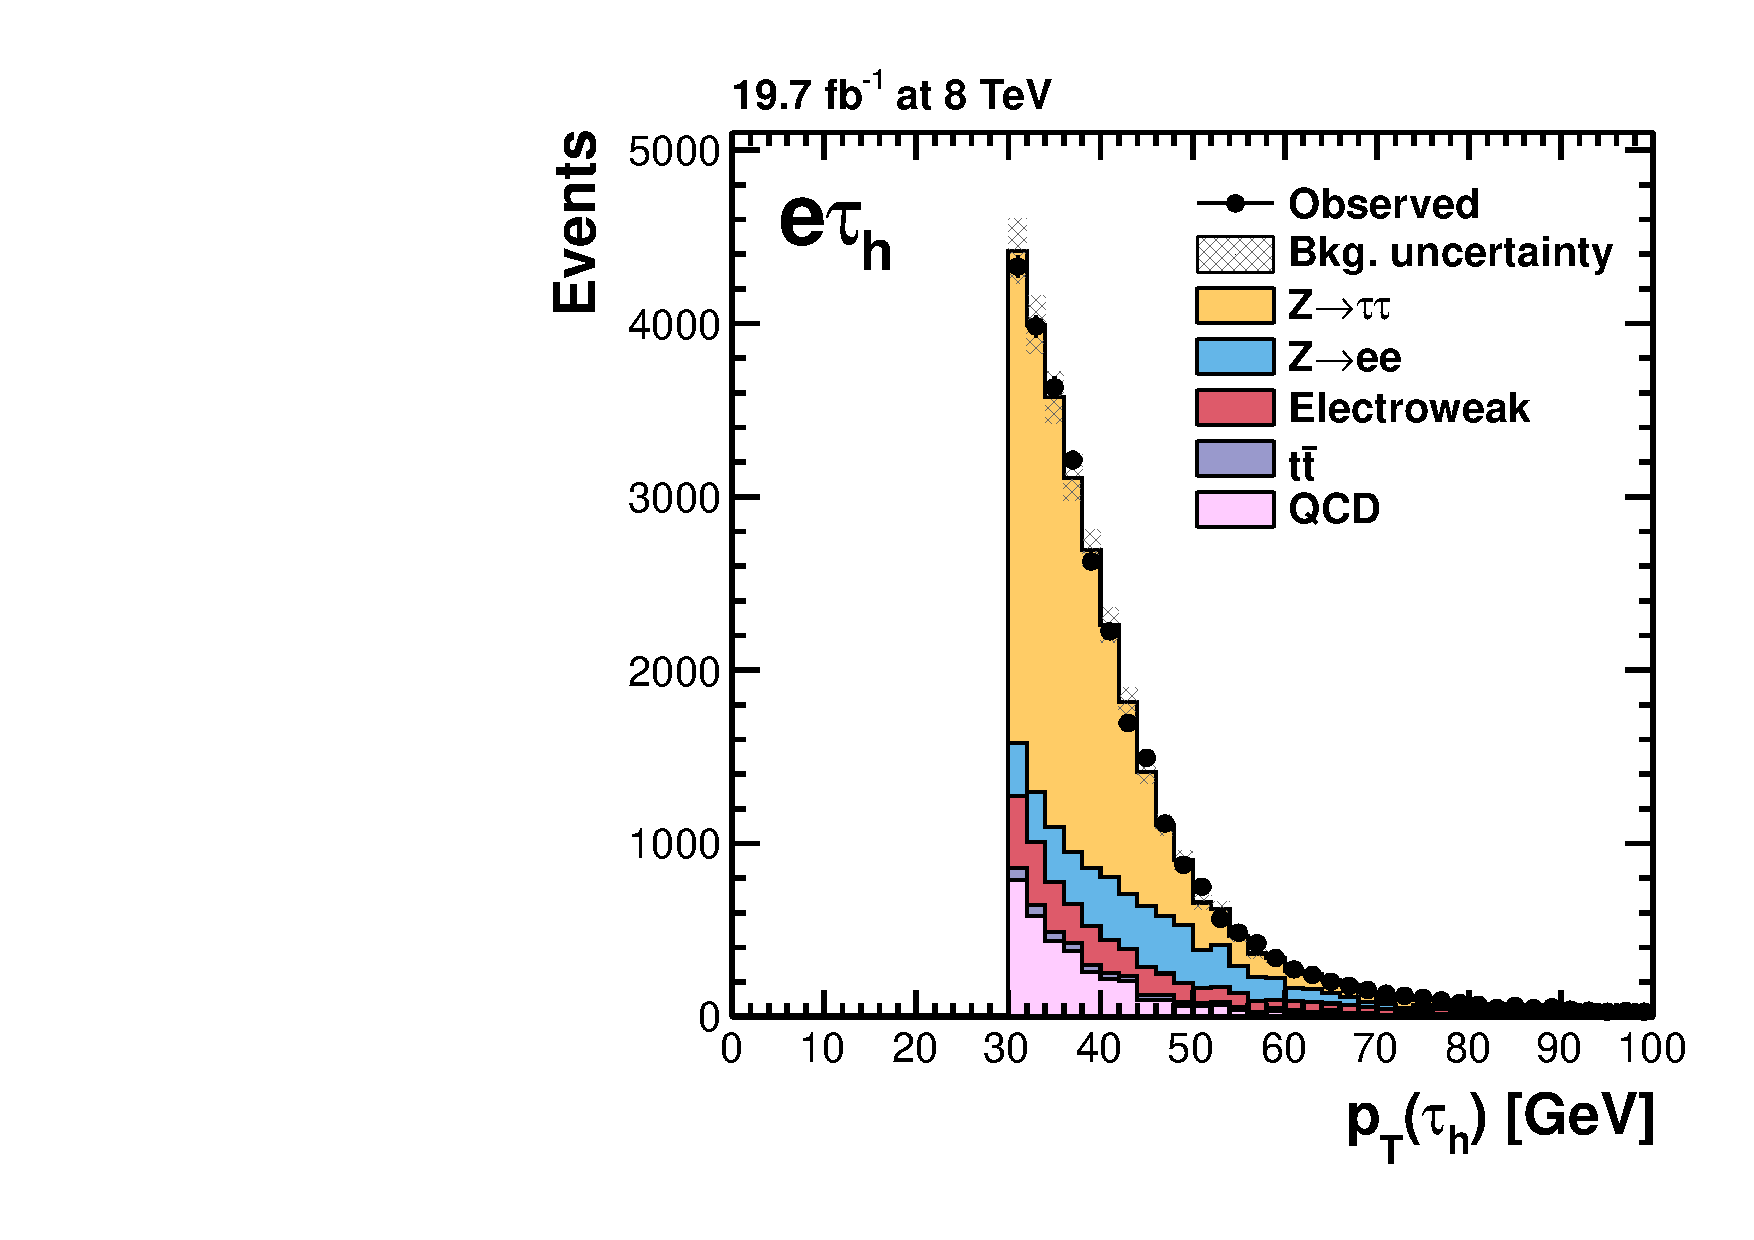
\includegraphics[width=0.5\textwidth]
      {plots/htt-sm/pt_2_inclusive_et_2012.pdf}}
\subfloat[]{
    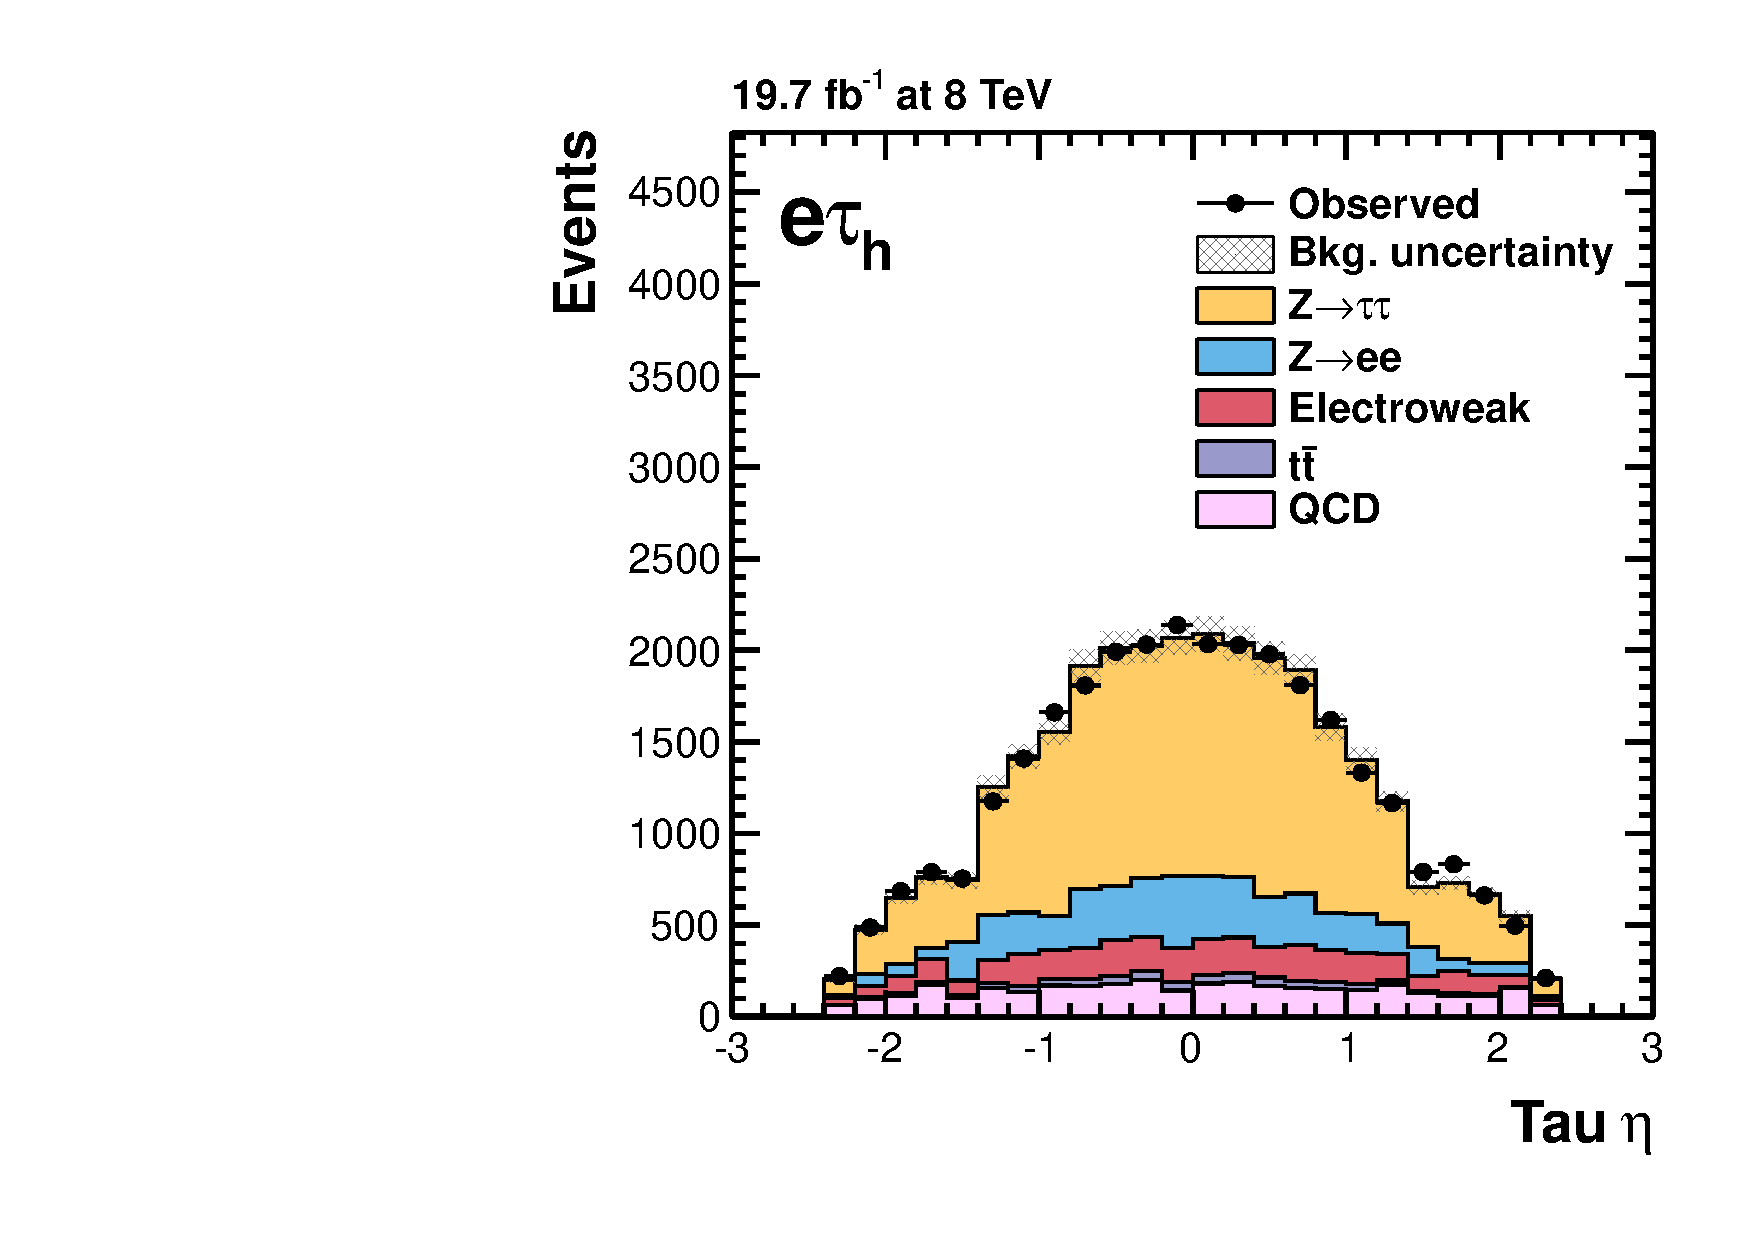
\includegraphics[width=0.5\textwidth] 
      {plots/htt-sm/eta_2_inclusive_et_2012.pdf}} 

\end{center}
\caption{
The $\pt$ and $\eta$ distribution for tau candidates in the $\etau$
channel.
}
\label{fig:etautaus}
\end{figure}

\subsection{Candidate Pair in the $\mutau$ Channel}

Events in the $\mutau$ channel are selected requiring an muon and hadronic tau
candidate. The muon is required to have $\pt$ larger than ($17~\GeV$)
$20~\GeV$ in (2011) 2012 data. In all data taking periods the $\eta$ requirement
on the muon is $|\eta| < 2.1$. The muon is required to pass tight muon ID as
defined in section \ref{sec:muons}. The isolation definition described in 
section \ref{sec:leptonisolation} is
applied with a threshold of 0.1. The muon must be compatible with
originating at the chosen \ac{PV}, and so the impact parameters in the
transverse and beam directions, $d_{xy}$ and $d_{z}$ respectively, must be
small. 

The hadronic tau has the same ID and isolation definition as described for the $\etau$
channel, with the exception of the anti-electron and anti-muon discriminators.
In the $\mutau$ channel a tight anti-muon discriminator and a loose
anti-electron discriminator are used. 

The muon and hadronic tau are required to be of opposite charge. 
The $\pt$ and $\eta$ distributions of the candidate pair in the
$\mutau$ channel are shown in figure \ref{fig:mutaumuons} for the muon and
\ref{fig:mutautaus} for the tau. 


\begin{figure}[htb]
\begin{center}
\subfloat[]{
    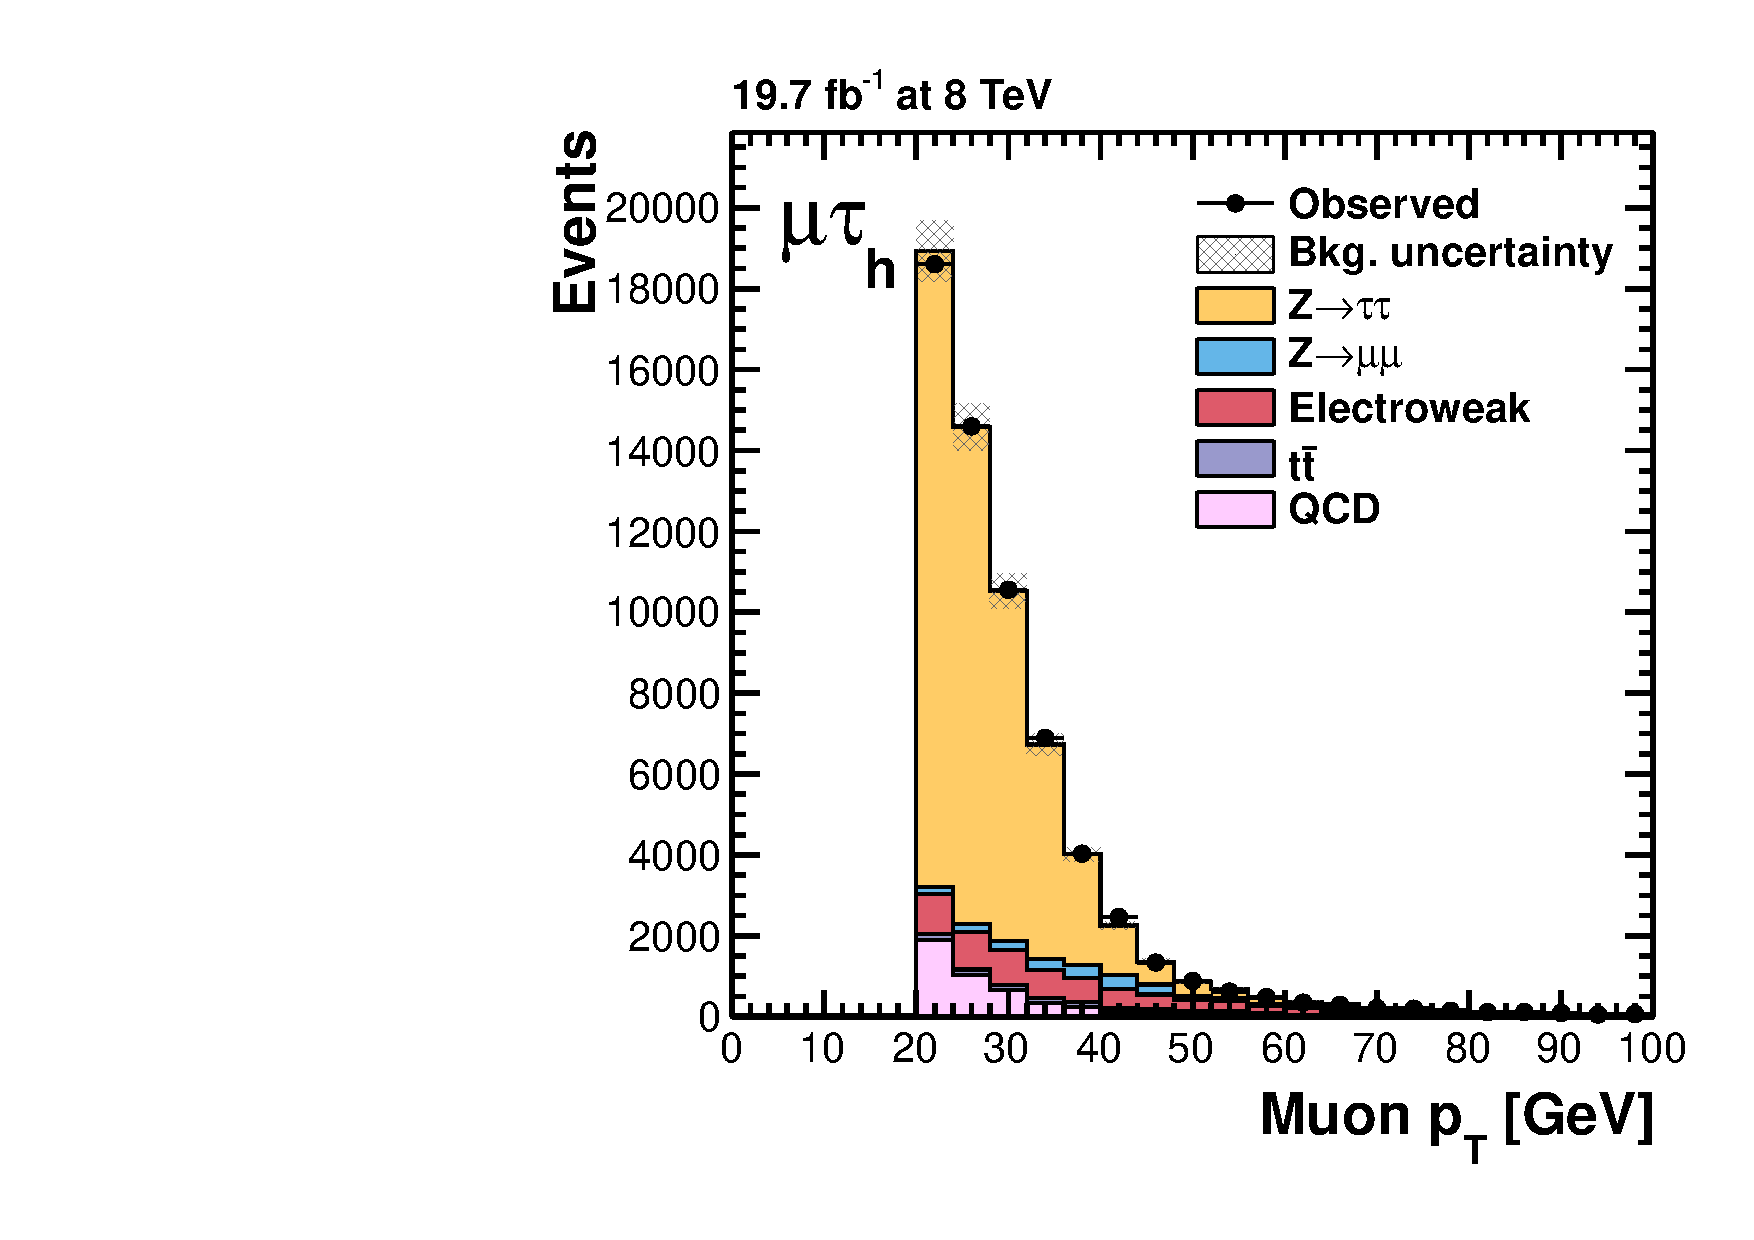
\includegraphics[width=0.5\textwidth]
      {plots/htt-sm/pt_1_inclusive_mt_2012.pdf}}
\subfloat[]{
    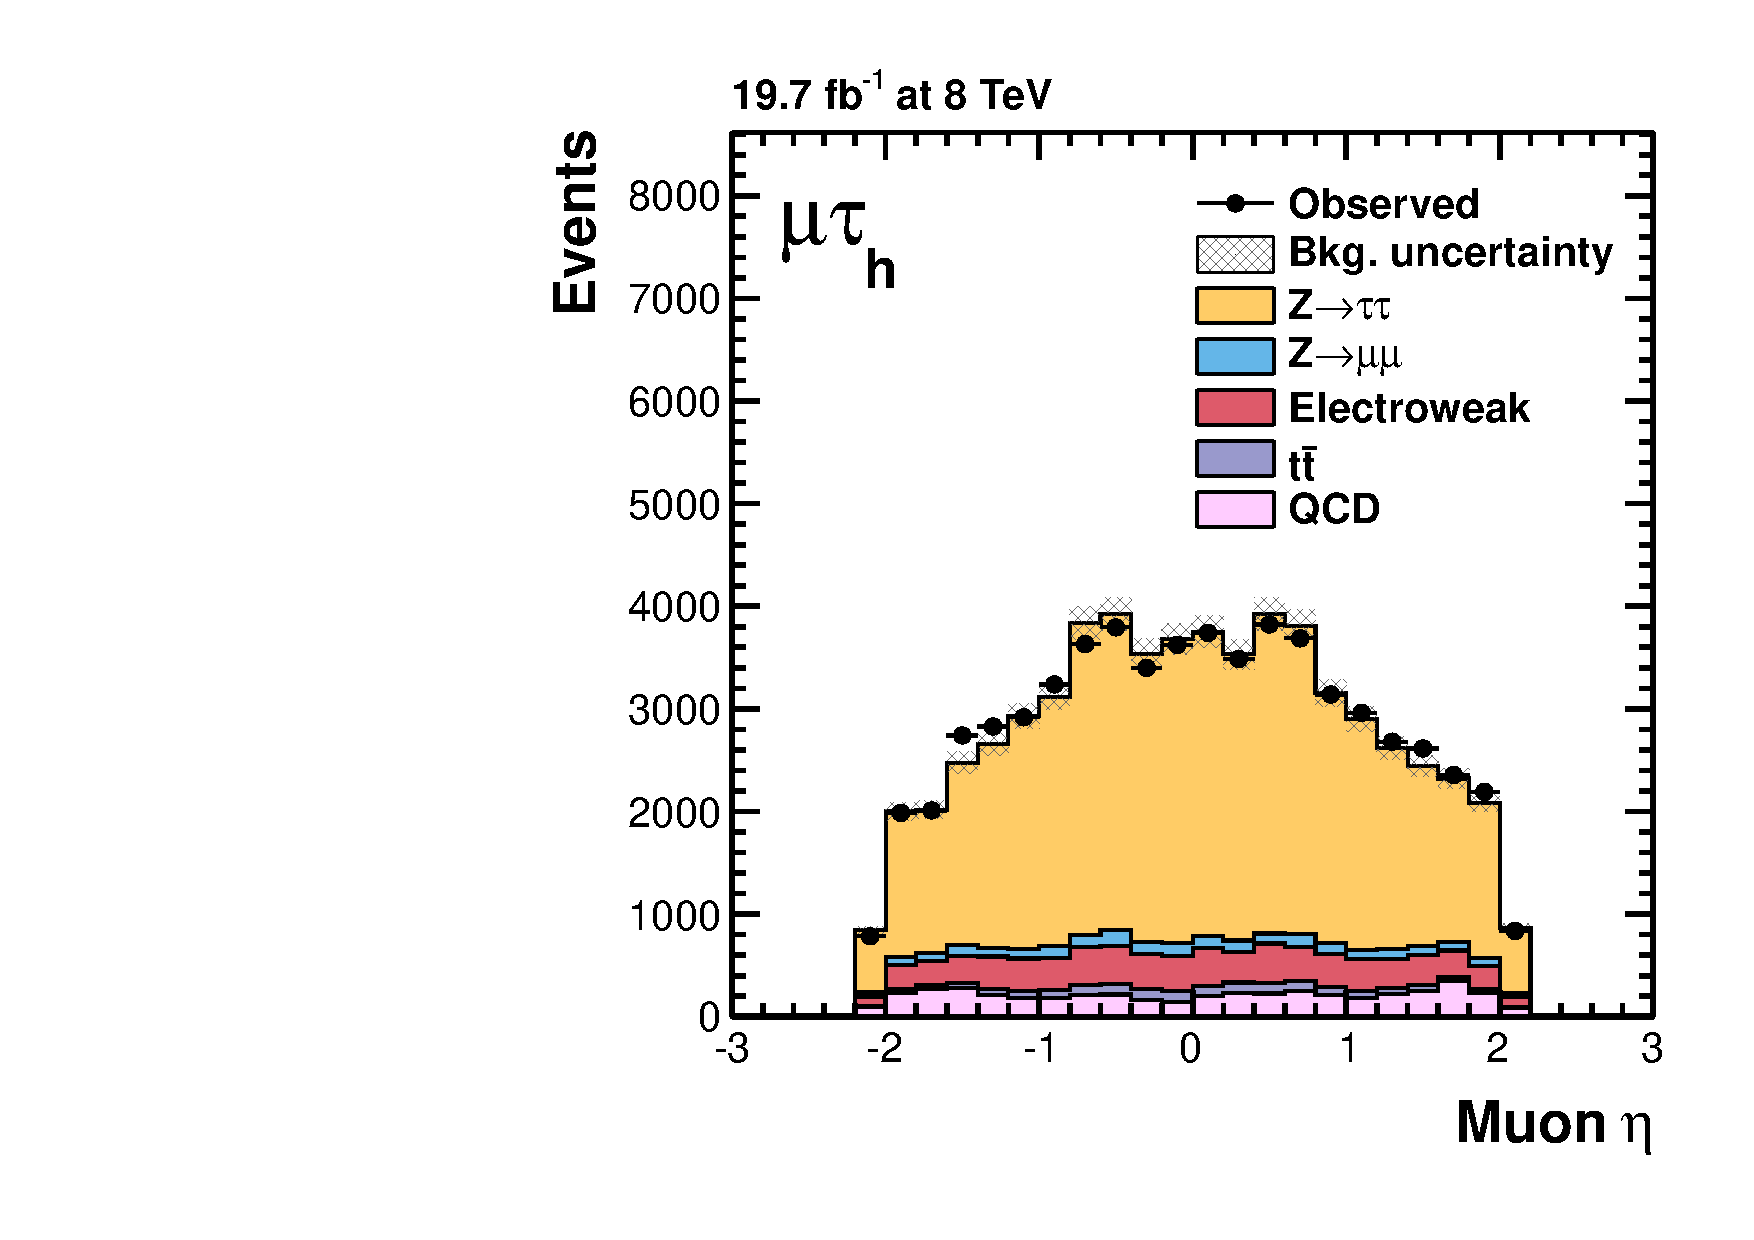
\includegraphics[width=0.5\textwidth] 
      {plots/htt-sm/eta_1_inclusive_mt_2012.pdf}} 

\end{center}
\caption{
The $\pt$ and $\eta$ distribution for muon candidates in the $\mutau$
channel.
}
\label{fig:mutaumuons}
\end{figure}


\begin{figure}[htb]
\begin{center}
\subfloat[]{
    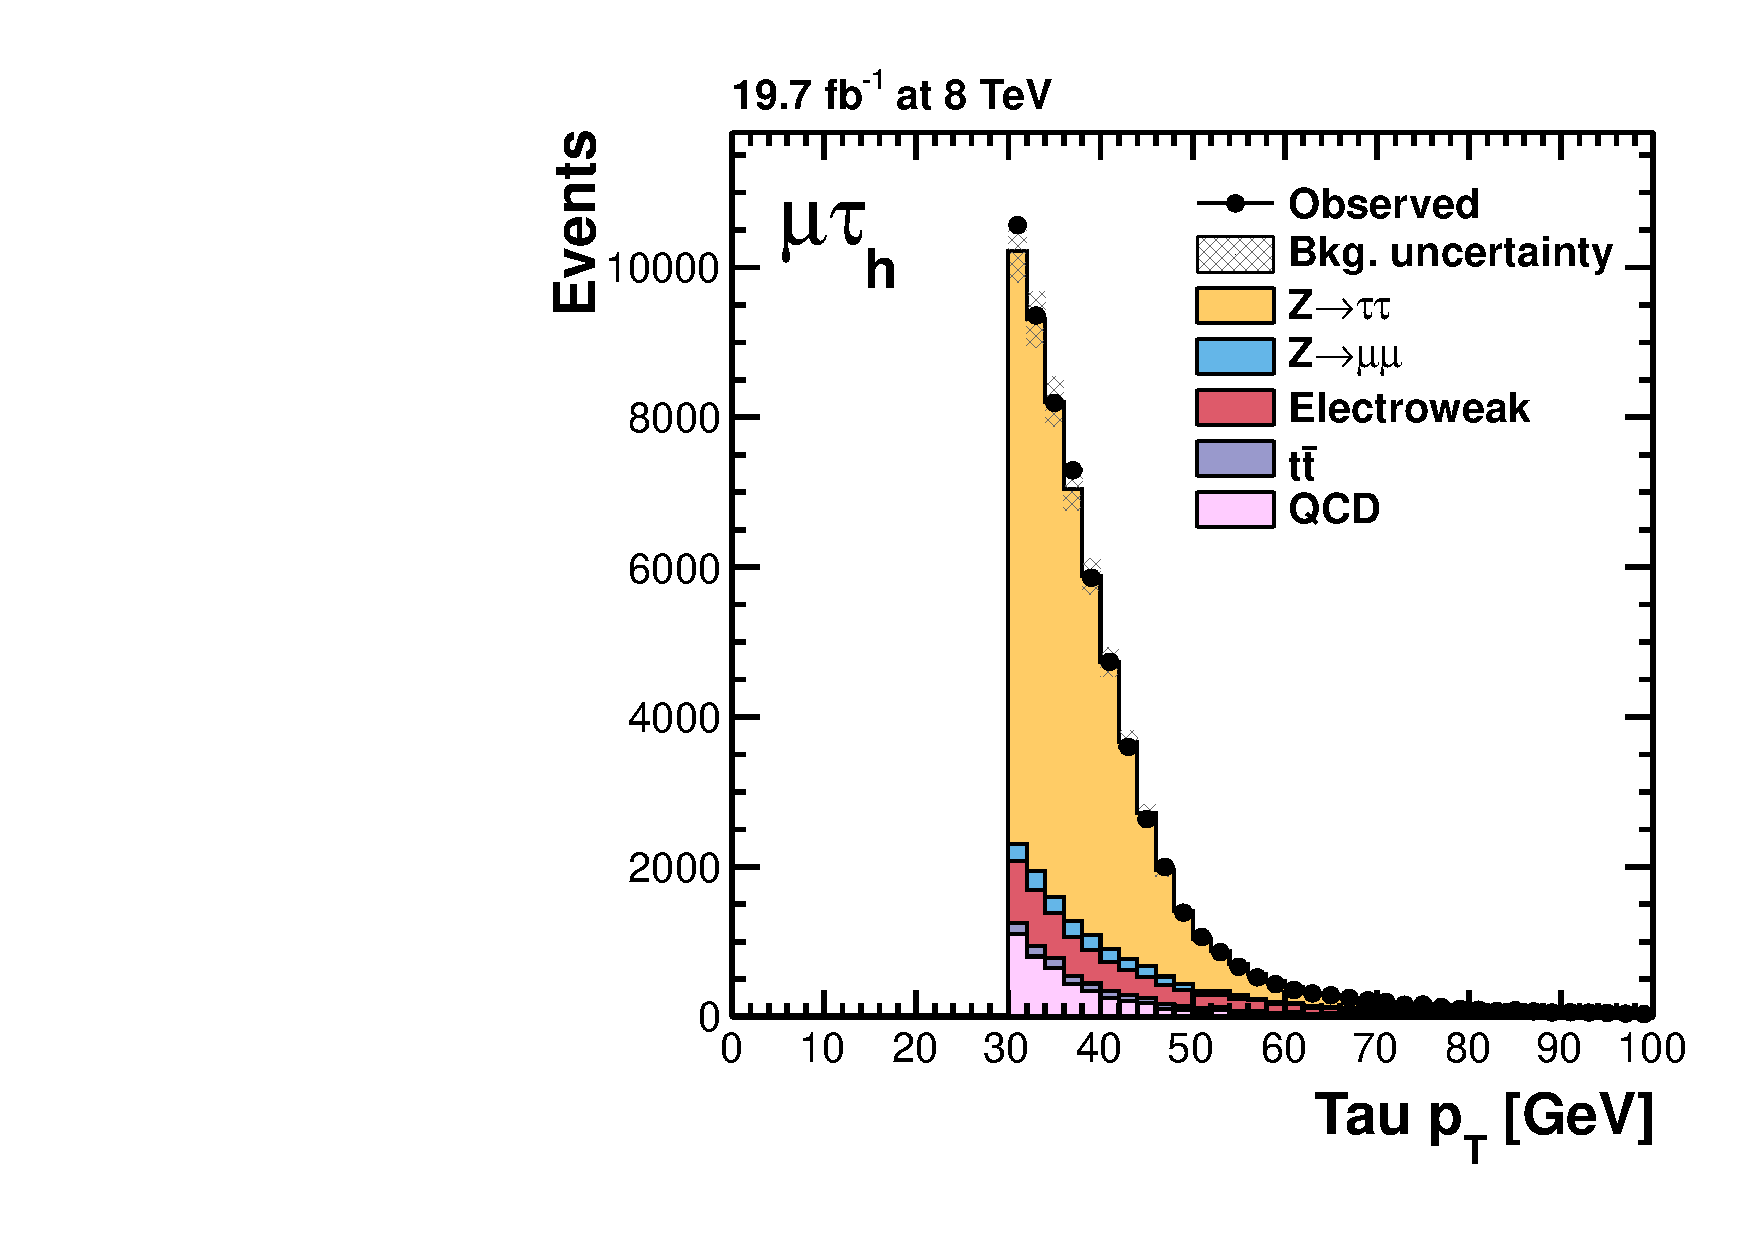
\includegraphics[width=0.5\textwidth]
      {plots/htt-sm/pt_2_inclusive_mt_2012.pdf}}
\subfloat[]{
    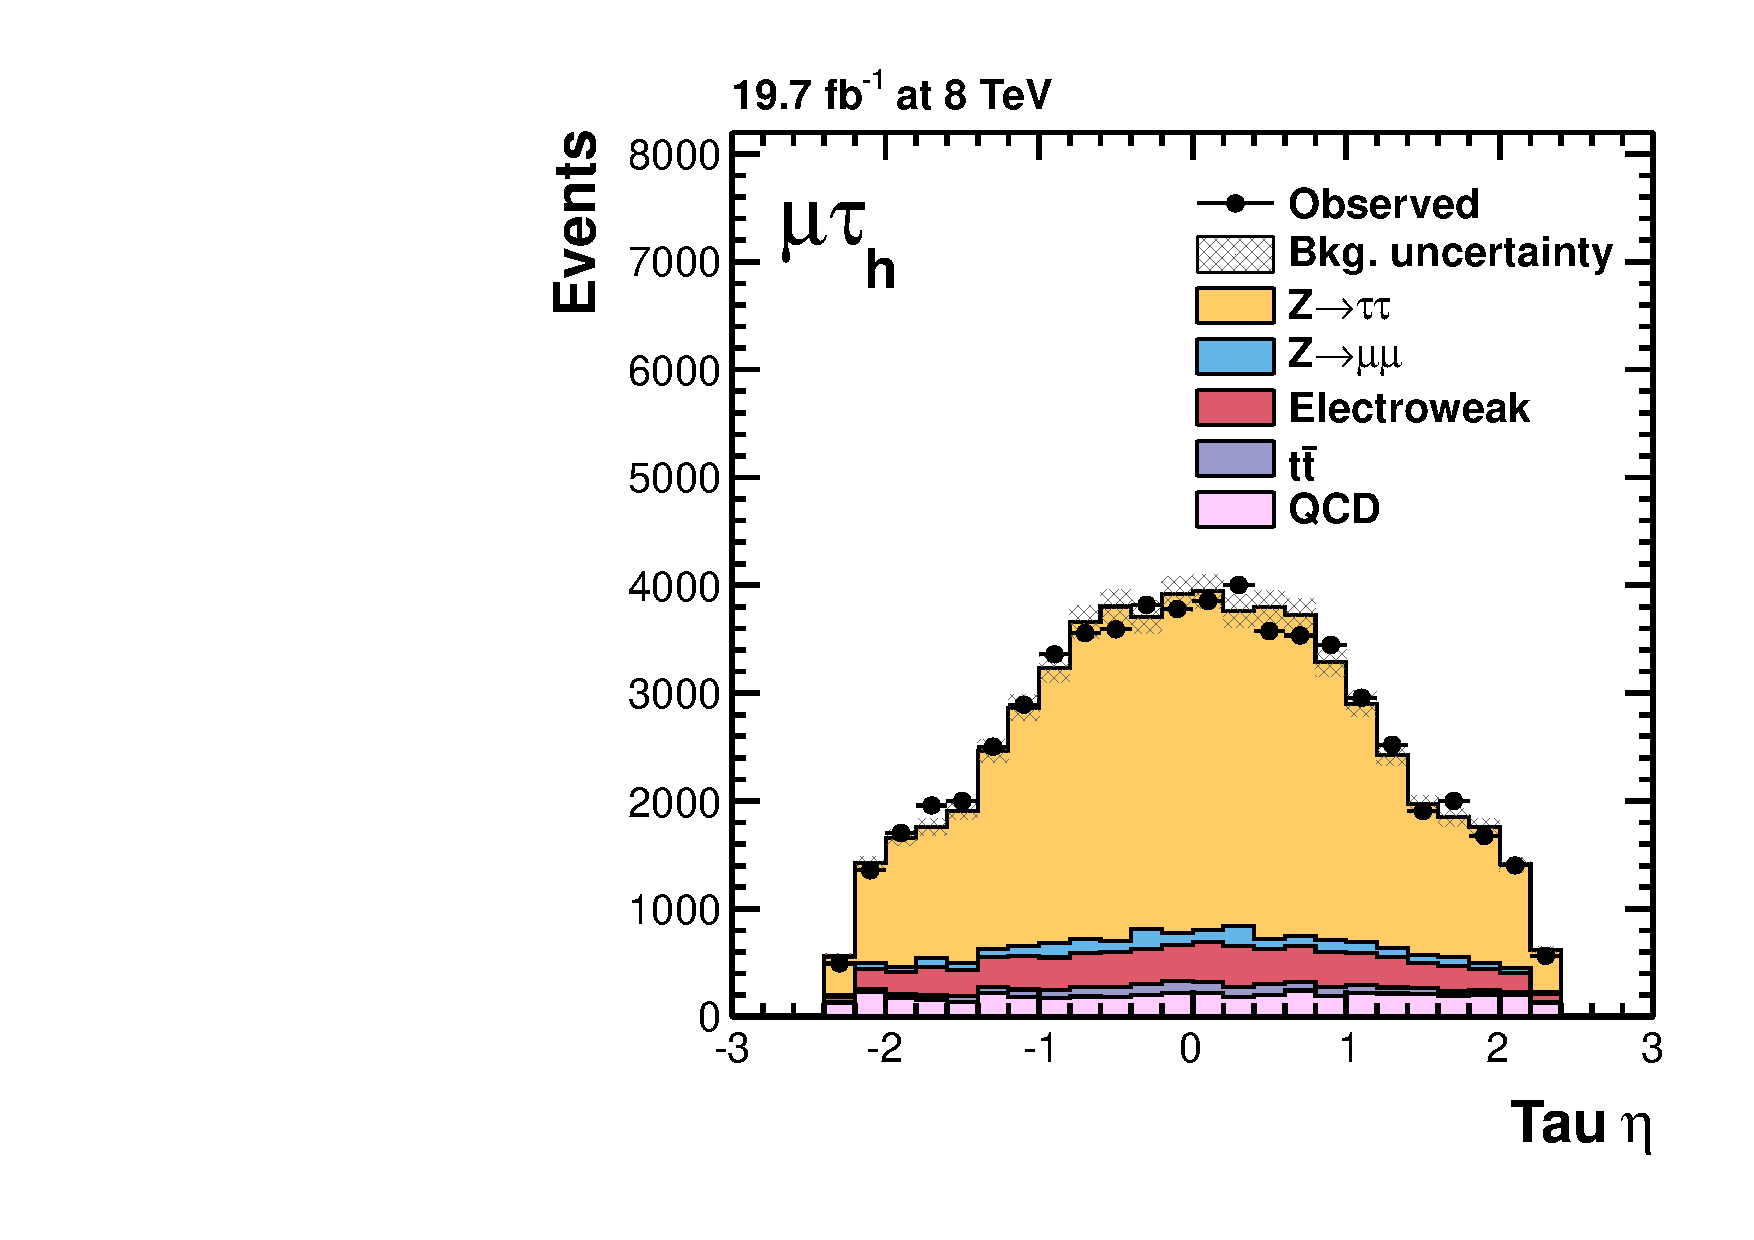
\includegraphics[width=0.5\textwidth] 
      {plots/htt-sm/eta_2_inclusive_mt_2012.pdf}} 

\end{center}
\caption{
The $\pt$ and $\eta$ distribution for tau candidates in the $\mutau$
channel.
}
\label{fig:mutautaus}
\end{figure}



\subsection{Extra lepton vetos}

\subsection{Topological Selection}

After selection of the candidate pair, a large background from $\WJets$ remains
in the $\etau$ and $\mutau$ channels, usually with the lepton from the $\PW$ and
a jet faking the hadronic tau. A useful quantity to reduce this background is
the transverse mass between the lepton and the $\MET$:

\begin{equation}
m_{\text{T}}\equiv\sqrt{2\pt^{\ell}\MET(1-\cos(\Delta\phi))},
\end{equation}

where $\pt{\ell}$ is the $\pt$ of the electron or muon and $\Delta\phi$ is the
difference in azimuthal angle between the lepton and the $\MET$. In real tau
events from $\PZ\to\Pgt\Pgt$ or $\PH\to\Pgt\Pgt$ the neutrinos in the $\Pgt$
decay tend to be produced collinearly with the visible products, whereas in
$\WJets$ events the neutrinos originate from the $\PW$ which has a much higher
mass than the $\Pgt$, and hence the neutrino is more likely to travel in the
opposite direction to the lepton in the transverse plane. Hence $\WJets$ events
have a higher transverse mass than signal events, and so a cut of
$m_{\text{T}}<30\,\GeV$ is found to reduce a large amount of $\WJets$ events
whilst still retaining a good signal efficiency.

Figure \ref{fig:transversemass} shows the distribution of $m_{\text{T}}$ for all
events in the $\mutau$ channel before the $m_{\text{T}}<30\,\GeV$ cut is
applied.

\begin{figure}[htb]
\begin{center}
\subfloat[]{
    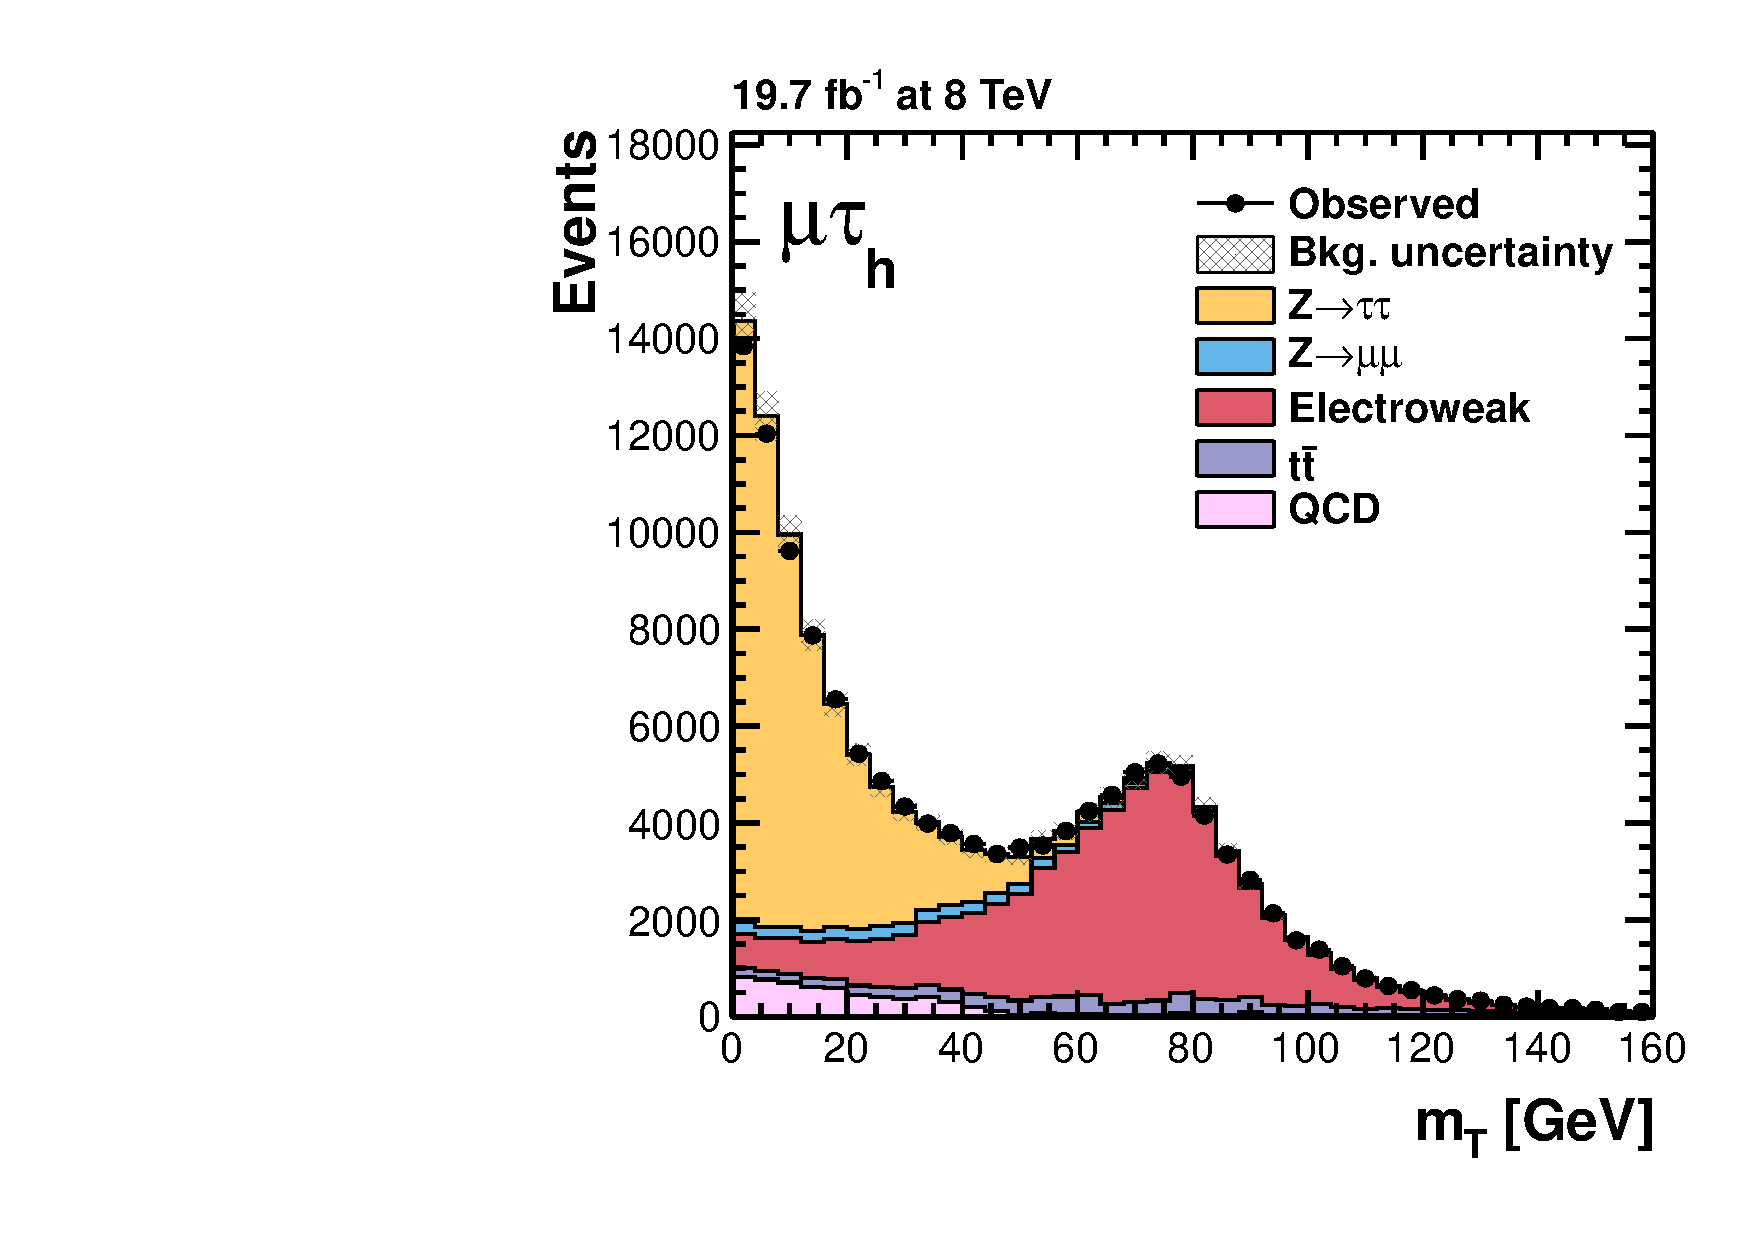
\includegraphics[width=0.5\textwidth]
      {plots/htt-sm/mt_1_inclusive_mt_2012.pdf}}

\end{center}
\caption{
 The transverse mass between the muon and the $\MET$ in the $\mutau$ channel.  
}
\label{fig:transversemass}
\end{figure}


\section{Event Categorisation}
\label{sec:eventcategorisation}

Events with a good candidate lepton and tau pair are further categorised in
order to group events which are more background-like or signal-like. The
categorisation uses properties consistent with the different production modes of
the Higgs boson as described in section \ref{sec:theory}. Figure
\ref{fig:categories} illustrates these categories for the $\mutau$ and $\etau$
channels.

\begin{figure}[htb]
\begin{center}
\subfloat[]{
    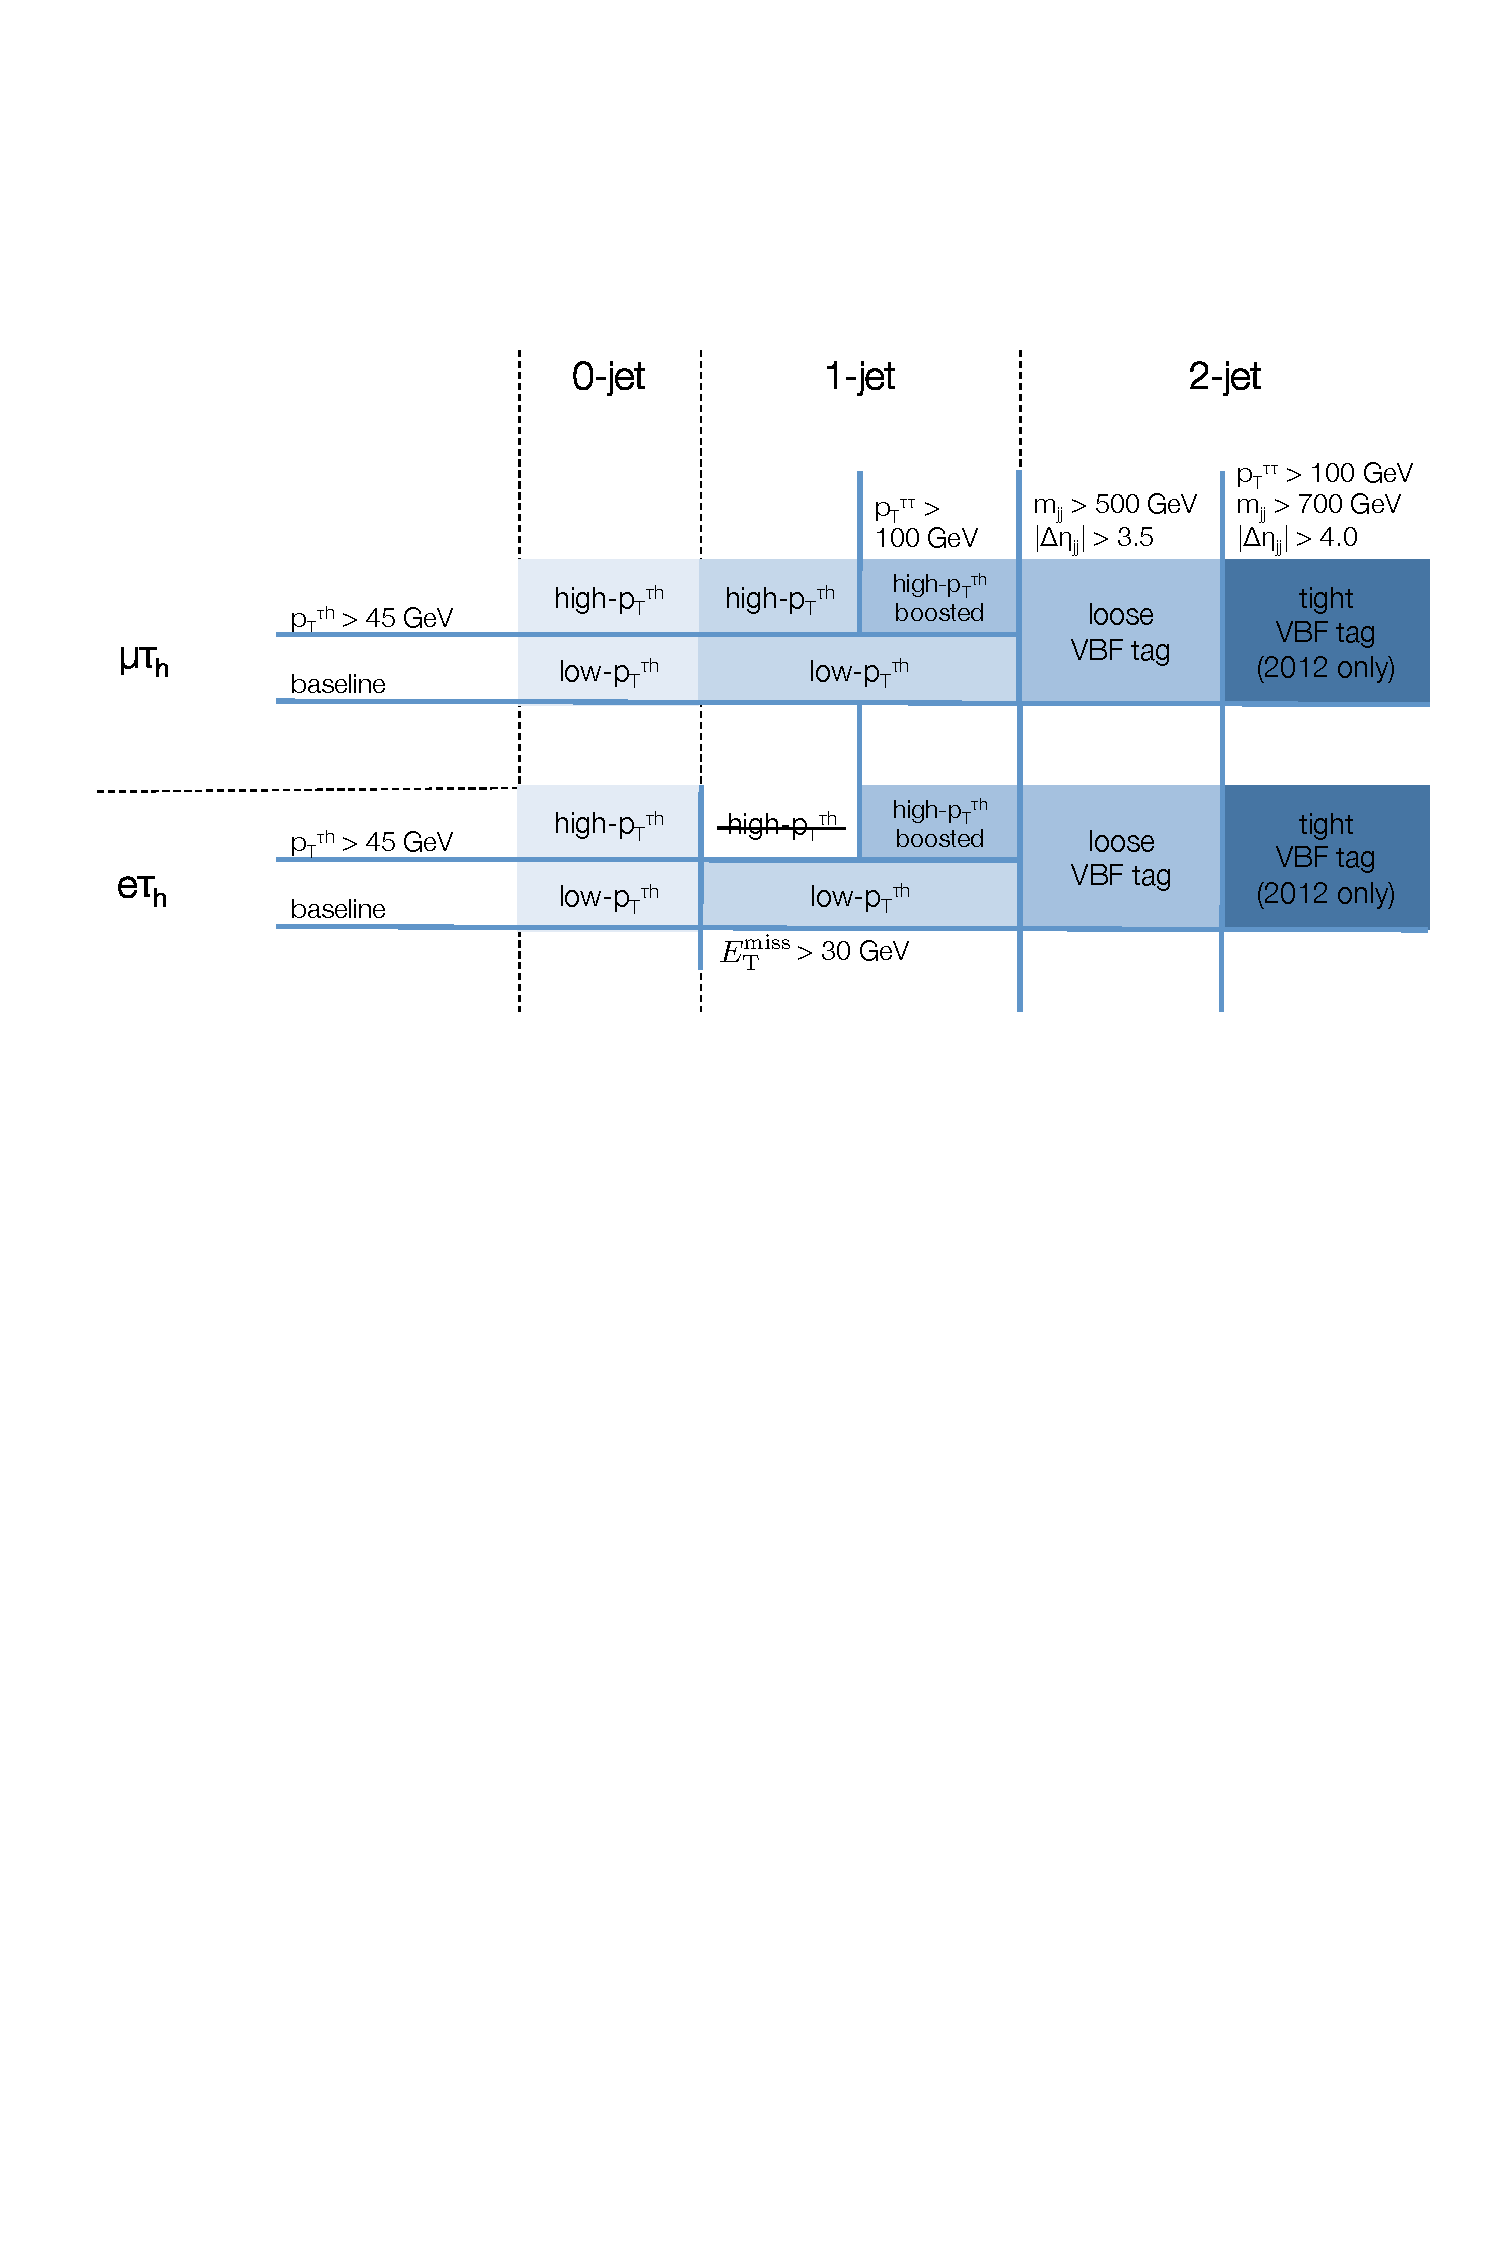
\includegraphics[width=0.7\textwidth]
      {plots/htt-sm/categories_2012.pdf}}

\end{center}
\caption{
 Categories used in the $\etau$ and $\mutau$ channels of the \ac{SM}
 $\HToTauTau$ analysis.  
}
\label{fig:transversemass}
\end{figure}
\section{Datasets and \ac{MC} samples}
\label{sec:dataandMC}


\section{Background Estimation}
\label{sec:backgrounds}

\subsection{Drell-Yan $\PZ \to\Pgt\Pgt$}
\label{sec:backgroundEstimation_Ztautau}

The $\PZ \to \Pgt\Pgt$ component is usually referred to as ``irreducible", due to its final
state involving two taus which only differ from the $\PH \to \Pgt\Pgt$ signal by
having an invariant mass closer to the mass of the Z instead of the Higgs. In
a final state with 2 taus and 2 b's, the $\PZ \to \Pgt\Pgt$ component is greatly reduced
by the requirement of at least 2 jets in the event, and still further reduced by
the b-tagging requirements and the mass constraint on m$_{\tau\tau}$.
However, it still remains an important background, in particular in the 2jet--0tag category. 

As described in section~\ref{sec:datasets_and_MonteCarloSamples}, an embedded
sample is used to better model this contribution. A Drell-Yan $\PZ \to\Pgt\Pgt$
sample is also used to esimate the overall yield of this background. 
The yield in each category is estimated by calculating the inclusive yield
using Drell-Yan $\PZ \to\Pgt\Pgt$ MC, and then scaling it by the efficiency for 
inclusive events to pass the category selection, which is estimated using the
embedded sample. The shape is then taken from the embedded sample within the
category selection.

To account for the known contamination of $t \bar{t}$ events in the embedded
samples, the embedded $t \bar{t}$ samples described in
section~\ref{sec:datasets_and_MonteCarloSamples} are used to evaluate the
expected contribution from such events, and then this is directly subtracted
from the $\PZ \to\Pgt\Pgt$ contribution.

\subsection{$\ttbar$}
\label{sec:backgroundEstimation_TT}

For the $t \bar{t}$ both shape and normalisation are taken from MC. Both are checked
against data by defining control regions which are at least 90$\%$ pure in
$t \bar{t}$. In the $\PH \to \Pgt\Pgt$ analysis, this is normally done using the
$\Pe\Pgm$ final state of the taus, events which are not used in this analysis
because of the large $t \bar{t}$ background after the 2 jet requirement. The control
region is defined with events passing the $\emu$ selection as defined in
\cite{HIG-13-004}, in addition to containing at least 2 jets, at least one b-tagged jet
and $\MET$ $>$ 80~$\GeV$. This control region has 91$\%$ $\ttbar$ purity.
An additional control region can be defined in the $\mu\tau_{had}$ and
$e\tau_{had}$ channels. Here, events with at least 2 b-tagged jets and $m_{T}$
$>$ 70~$\GeV$ are used. This control region has lower statistics than the $\emu$ one
but a higher $t \bar{t}$ purity of 95$\%$. The plots showing some important variables
in these control regions can be found in figure~\ref{fig:backgroundsTTControl}.

A reweighting is applied to $t \bar{t}$ events. The correction has been developed by the Top
group to better match the top quark $P_{T}$ distribution observed in data~\cite{TopPtReweighting}. 

\subsection{$\WJets$}
\label{sec:backgroundEstimation_WplusJets}

W plus jets is a background in this analysis where there is a real electron or
muon from the W and one of the associated jets fakes a hadronic tau. This
background is largely reduced by the $m_{T}$ $<$ 30 GeV cut described in
section~\ref{sec:eventSelection}. To estimate the remaining contribution the
events with $m_{T}$ $>$ 70 GeV are used, which are dominated by W+jets and $t
\bar{t}$
events. This sideband is used to estimate the sideband normalisation of the W+jets, by
subtracting all other backgrounds from data and taking the rest to be W.
An extrapolation factor, to take the estimate from the high m$_{T}$ region to
give an estimate in the signal region with $m_{T}$ $<$ 30 GeV, is calculated from MC.

In the 2jet--2tag category, where there is a much larger contribution from $t
\bar{t}$ events in the $m_{T}$ $>$ 70 GeV region, the control region is instead
defined as 60 $<$ $m_{T}$ $<$ 120 GeV, which gives a larger amount of statistics for
the W estimate after subtracting the other backgrounds.

The shape of the W is taken from MC in each category. Due to the low event statistics in the
categories, the category selections for the 2jet--1tag and 2jet--2tag W
estimates are relaxed to include b-tagged jets passing the loose CSV working point 
instead of the medium.

\subsection{QCD}
\label{sec:backgroundEstimation_QCD}

QCD is estimated entirely from data. It is expected that the contribution of
same sign and opposite sign events from QCD is roughly the same. Thus the same
sign data is used with all other backgrounds subtracted, to predict the rate of
QCD in the opposite sign events. For the background subtraction, the W+jets is
estimated as described in the previous section and all other background
contributions are estimated from MC. The opposite sign/same sign rates from QCD
are in fact not exactly the same, and an extrapolation factor of 1.06, measured
using data with the electron/muon isolation inverted, is applied to correct for
this.

Due to the low statistics in the categories, it is necessary to define another
sideband from which to extract the QCD estimate. This is done by inverting the
electron/muon isolation in same-sign events. In the 2jet--2tag category, this
anti-isolated sideband is used to calculate an extrapolation factor from events
with at least 2 jets to events passing the full 2jet--2tag selection. Then this
extrapolation factor is used to scale the normalisation of the same-sign
subtracted data in events with at least 2 jets.

The anti-isolated sideband is also used for the shapes. For the 2jet--0tag
category, the shape is directly taken from the anti-isolated data passing the
full category selection. The shapes for the 2jet--1tag
and 2jet--2tag categories are taken from the anti-isolated data with a 
looser category definition. This looser definition is the same as that used in
the W estimation, where the b-tag working point is loosened to the loose CSV
working point instead of the medium.

\subsection{Other backgrounds}
The remaining backgrounds are from $\PZ \to \ell\ell$, diboson and single top.
Both the normalisation and shapes of these backgrounds are estimated using MC.
The contributions from these backgrounds are much smaller.
The contribution of $Z/\gamma^{*} \to ee$ background to the $e\tau_{had}$ channel
is additionally corrected by $e \to \tau_{had}$ fake--rate Monte Carlo--to--data
scale--factors.

\section{Data/MC Correction Factors}
\label{sec:datamcfactors}

Whilst data-driven methods are used wherever possible, MC is still
relied on in predicting expected shapes and yields of signal and backgrounds.
As such is it important that the MC is corrected for
any effects which are known to be imperfectly modeled. For ID, isolation and
trigger efficiencies of the candidates in the analysis, the \ac{MC} is corrected
for measured differences in the efficiency in data and \ac{MC}.

This section documents measurements of these efficiences for the light leptons
of the $\etau$ and $\mutau$ channels. This is done using a ``tag and probe" method.
The tag and probe method makes use of a well known and measured resonance decaying
into a light lepton pair, in this case $\PZ\to\Pe\Pe$ or $\PZ\to\Pmu\Pmu$, 
in which one the light leptons is assigned as the `tag' and one is the `probe'. 
The tag is constrained by a very tight selection such that it is known with near 
certainty to be a real electron/muon. The probe is subject to a looser selection, 
but only tag/probe pairs with a
combined invariant mass close to the $\PZ$ mass are used. This ensures that the
prove is also an electron/muon with high probabiliy. Then the probe can be 
subjected to further cuts or constraints to measure the efficiency of such a 
selection to select real leptons.

The invariant mass distributions of the tag and probe events are used to extract
the different
selection efficiencies. A simultaneous fit of the mass shapes is performed, and
the ratio of the integral of the fitted $\PZ$ signal in the pass and fail
distributions is used to extract the efficiency. To account for any background
to the real $\PZ$ events, signal and background are both accounted for in the
fit.

The electron/muon ID efficiency is measured with a reconstructed
electron/muon as the probe. Then the electron/muon isolation efficiency is measured
with a probe which already fulfills the full ID selection criteria. 

The efficiencies for combined ID and isolation are shown in Figures
\ref{fig:electronIdIso} and \ref{fig:muonIdIso}, measured in the complete 2012
dataset and PU weighted MC, as a function of the lepton $\eta$ and $\pt$.
The scale factor which is used in the analysis is given by the ratio of the
measured efficiency in data (black) and MC (red), and is evaluated separately in
selected $\pt$ and $\eta$ bins.

\begin{figure}[h!]
\subfloat[]{
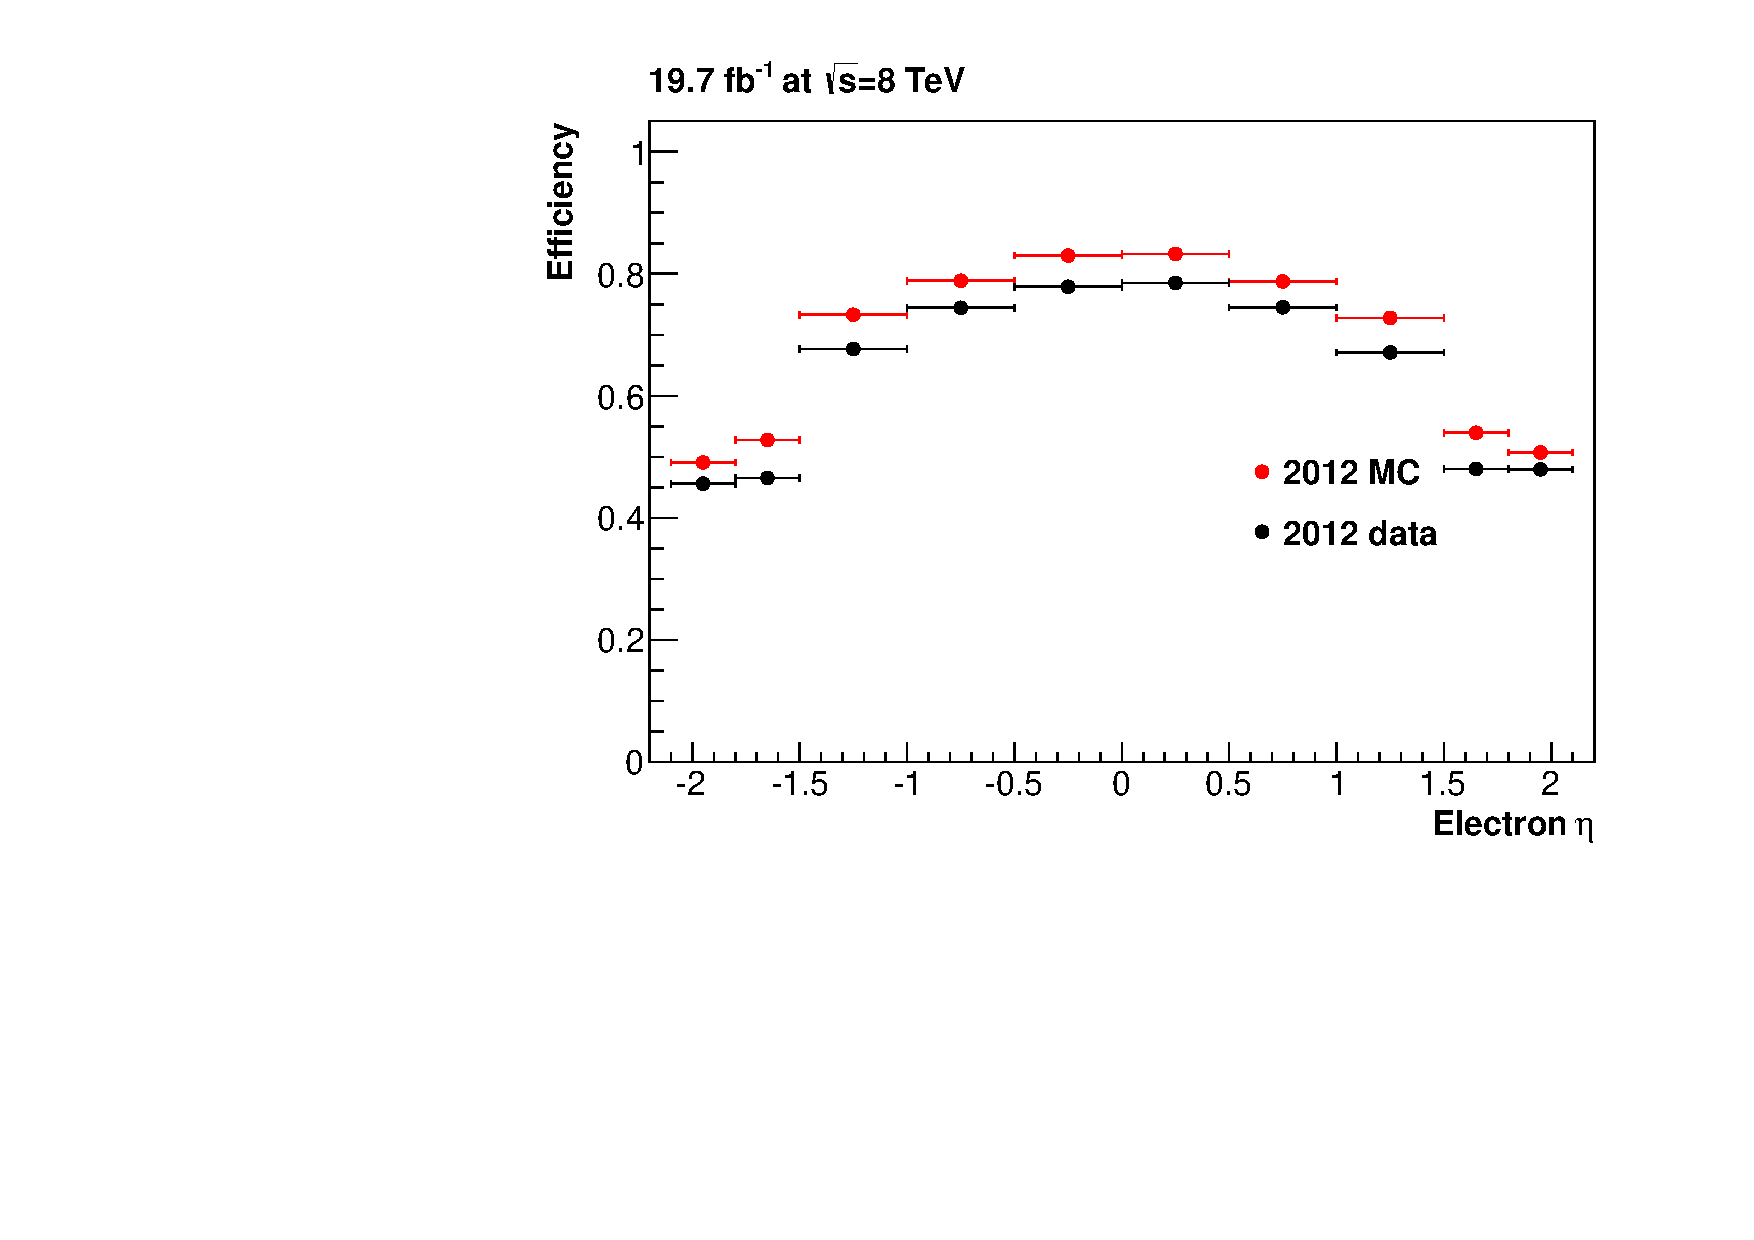
\includegraphics[width=0.5\textwidth]{plots/TagAndProbe/ElectronIdIsoEta2012DatavsMC.pdf}}
\subfloat[]{
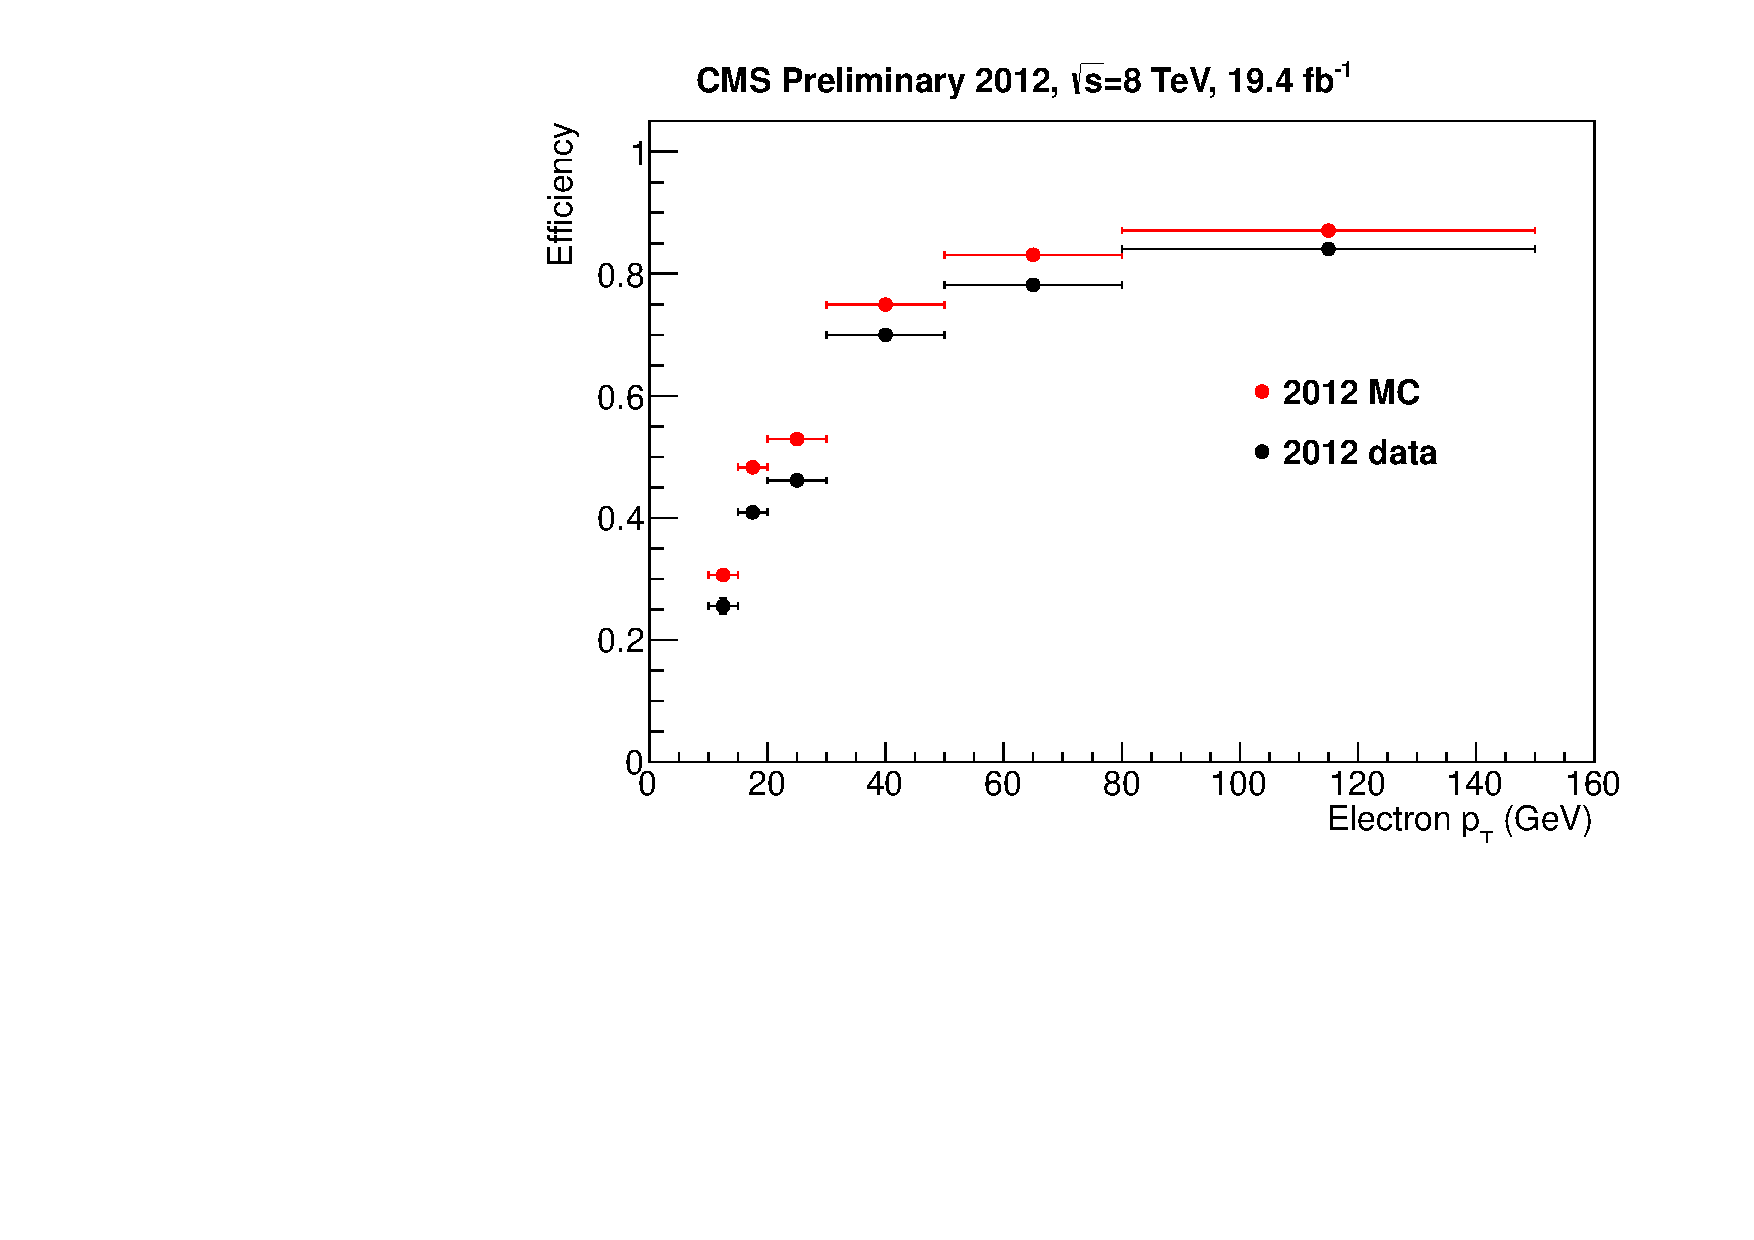
\includegraphics[width=0.5\textwidth]{plots/TagAndProbe/ElectronIdIsoPT2012DatavsMC.pdf}}
\caption{Combined electron ID and isolation efficiency in data and MC as a
function of (left) $\eta$ and (right) $\pt$}
\label{fig:electronIdIso}
\end{figure}

\begin{figure}[h!]
\subfloat[]{
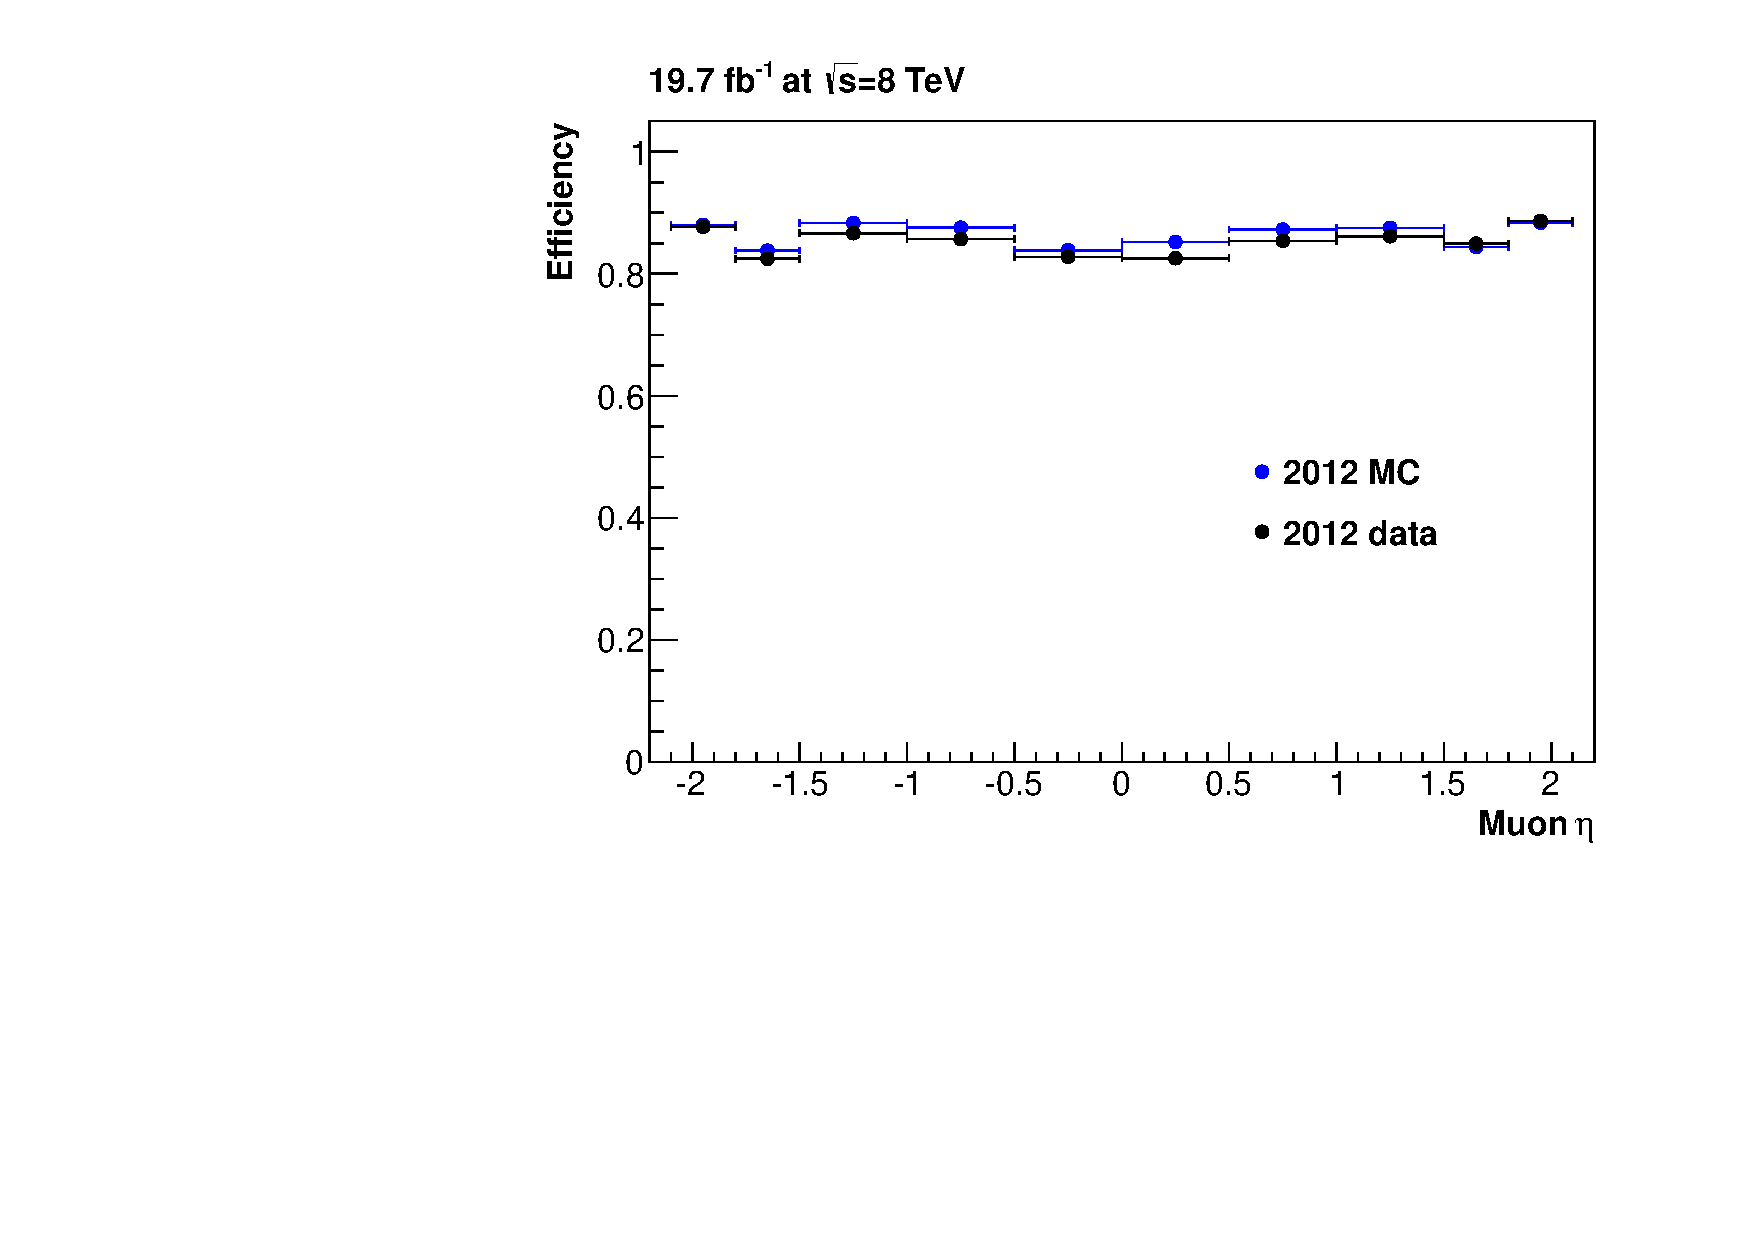
\includegraphics[width=0.5\textwidth]{plots/TagAndProbe/MuonIdIsoEta2012DatavsMC.pdf}}
\subfloat[]{
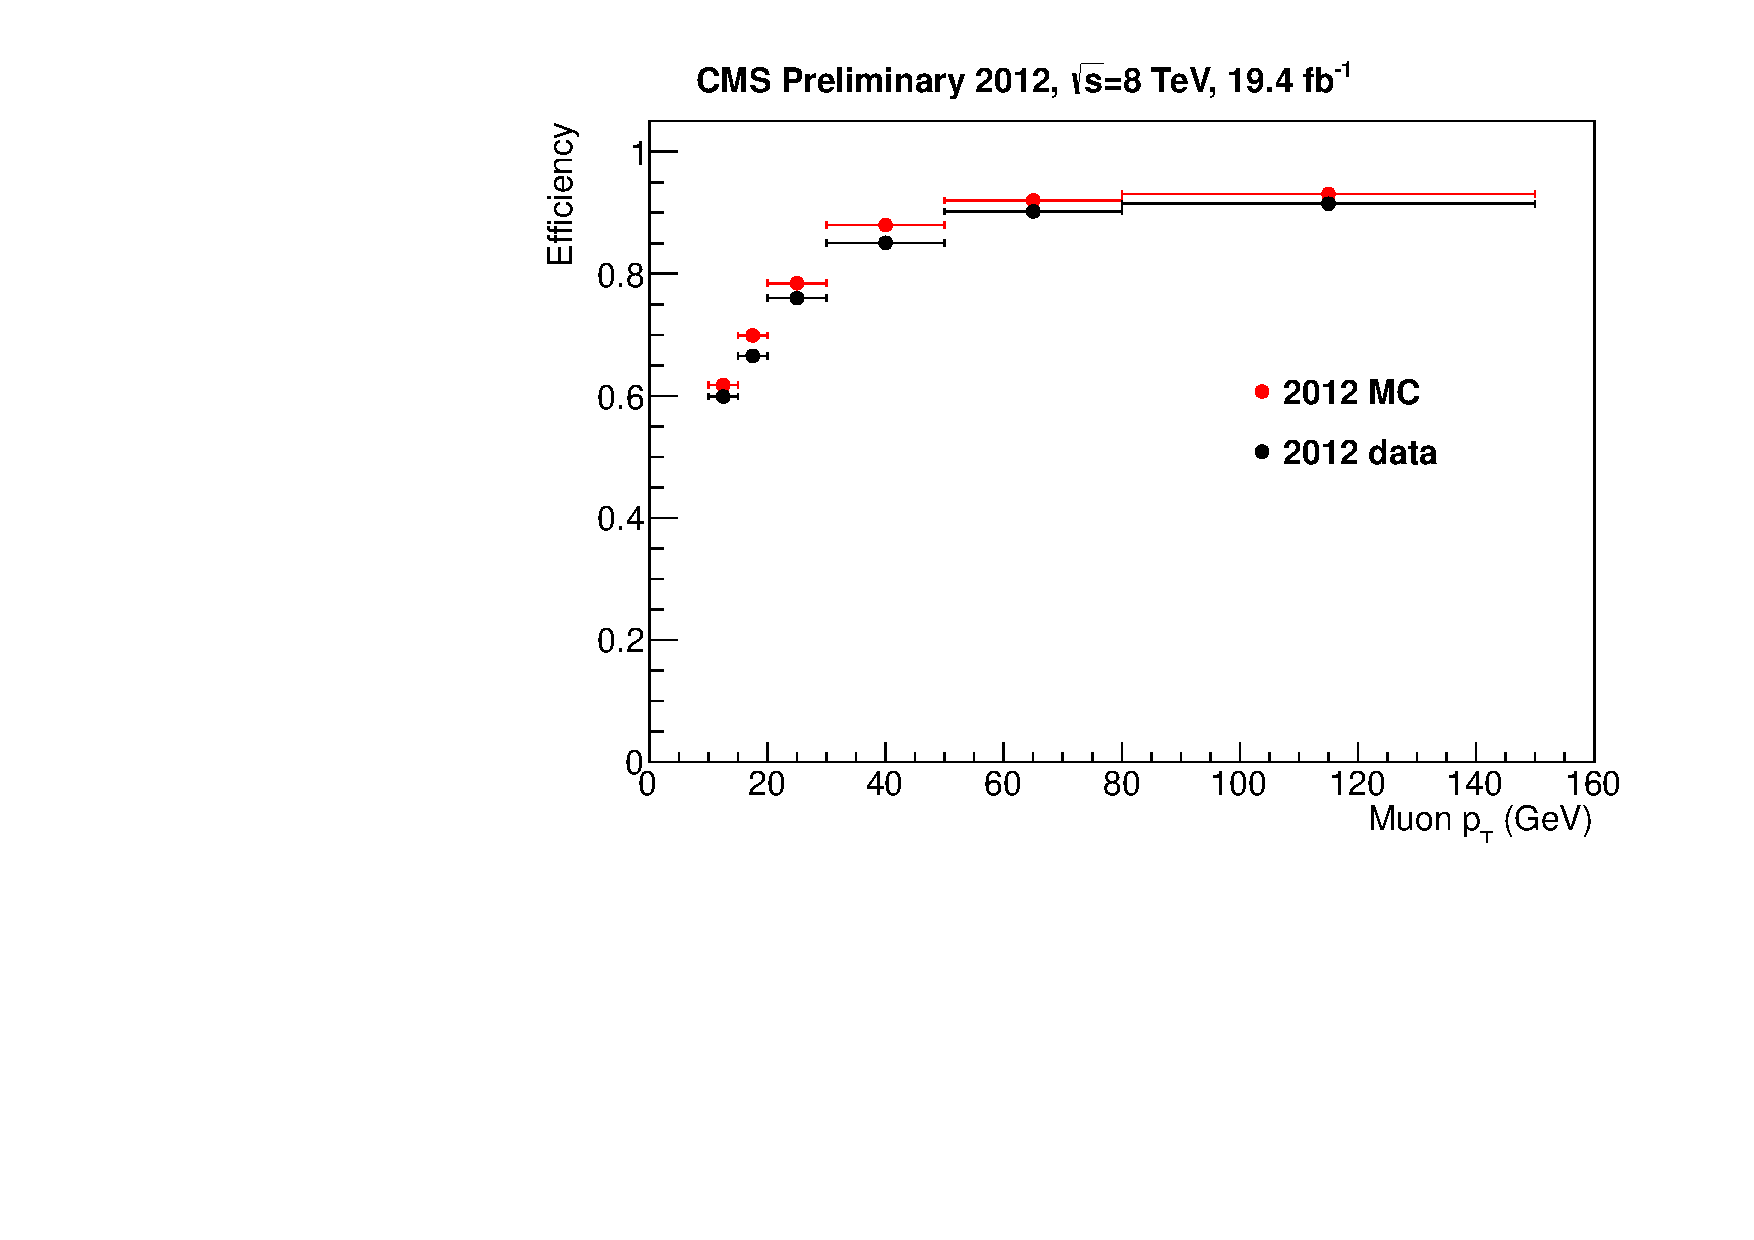
\includegraphics[width=0.5\textwidth]{plots/TagAndProbe/MuonIdIsoPT2012DatavsMC.pdf}}
\caption{Combined muon ID and isolation efficiency in data and MC as a function
of (left) $\eta$ and (right) $\pt$}
\label{fig:muonIdIso}
\end{figure}

\noindent The same method can be used to measure the efficiencies of the trigger
in data and MC. In this case a probe is used which has already passed both ID
and isolation, and the passing probe condition is that the lepton is responsible
for firing the lepton leg of the lepton+tau trigger. Figures
\ref{fig:electrontrg} and \ref{fig:muontrg} show the trigger efficiency as a
function of p$_{\rm{T}}$ measured in both 2012 data and MC. For the
electrons, the trigger is measured separately in the barrel and endcap
regions, which correspond to $|\eta| < 1.479$ and $|\eta| > 1.479$
respectively. For the muons, the trigger is measured in 3 regions, corresponding
to .

\begin{figure}[h!]
\subfloat[]{
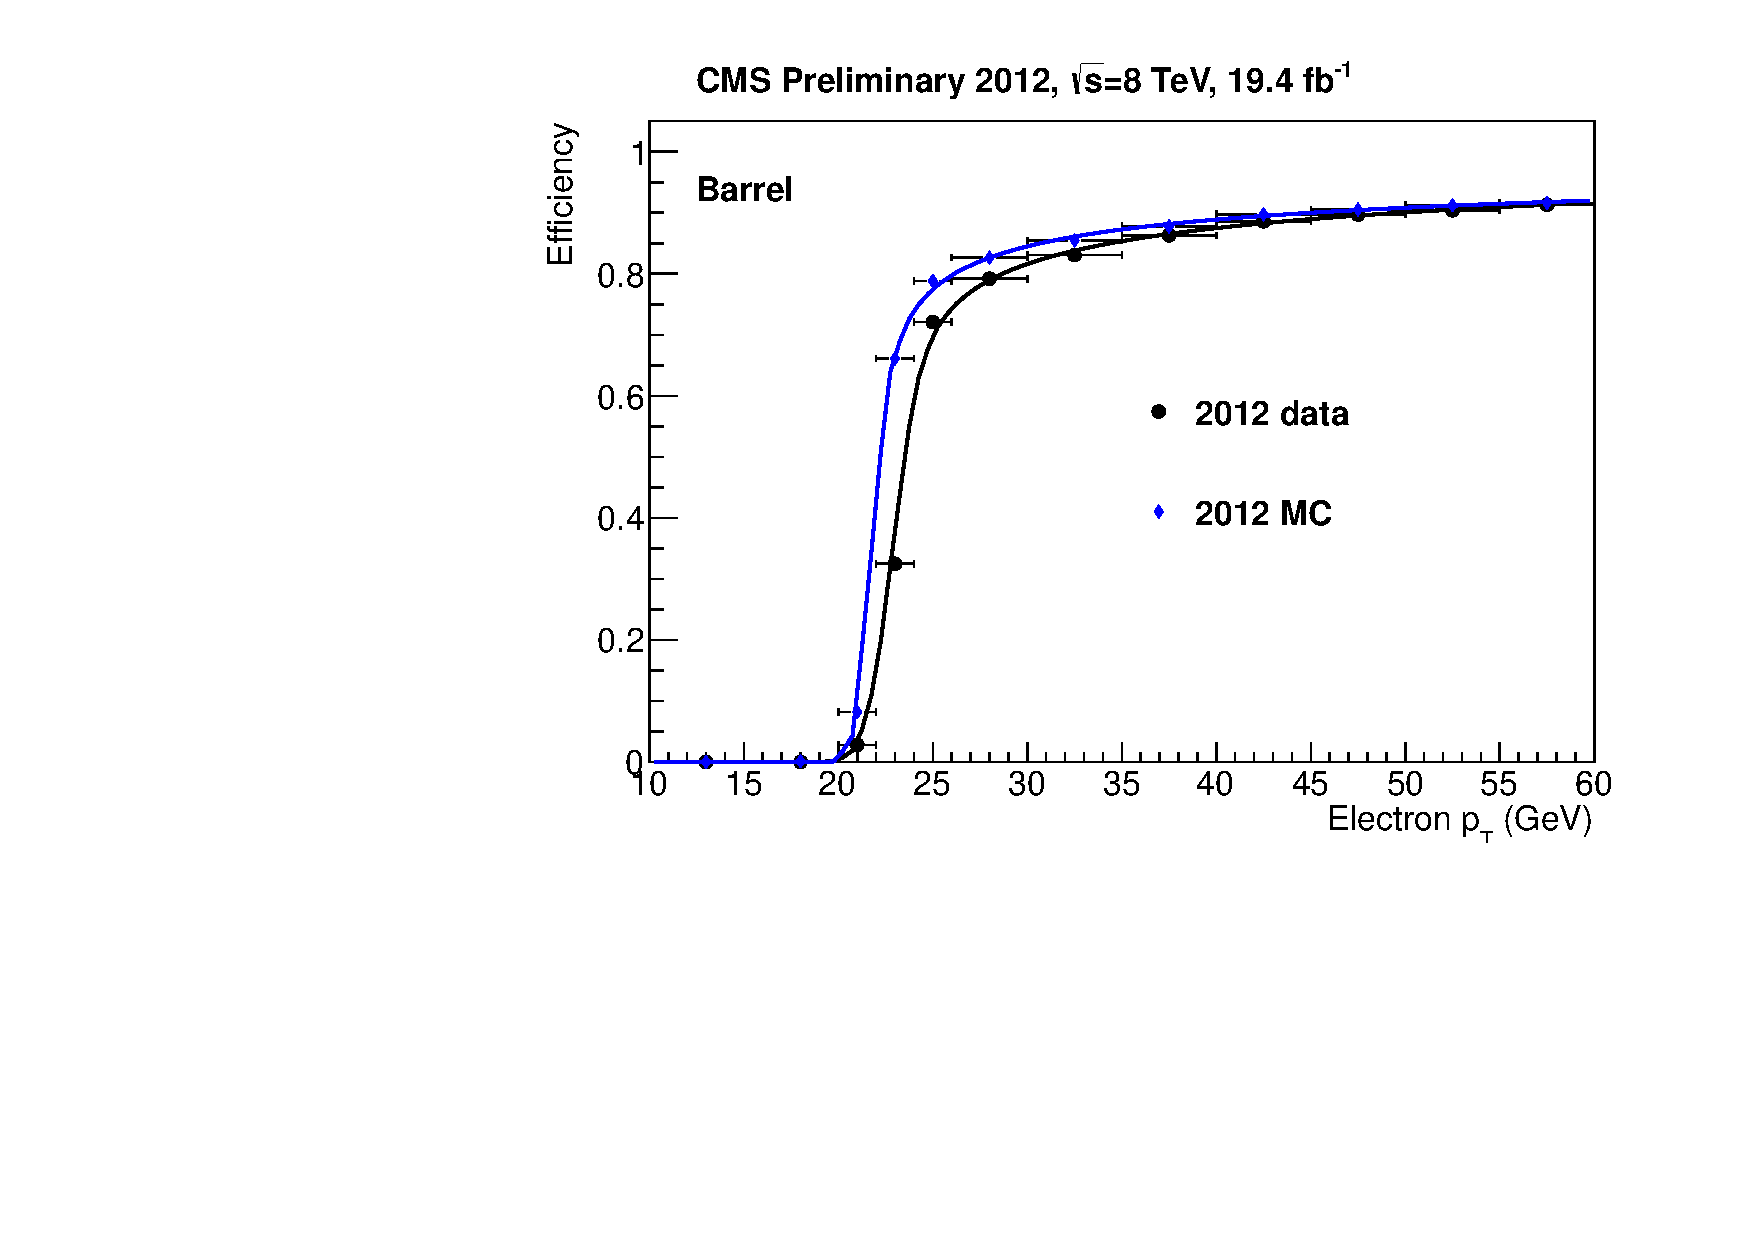
\includegraphics[width=0.5\textwidth]{plots/TagAndProbe/ElectronBarrel2012DatavsMC.pdf}}
\subfloat[]{
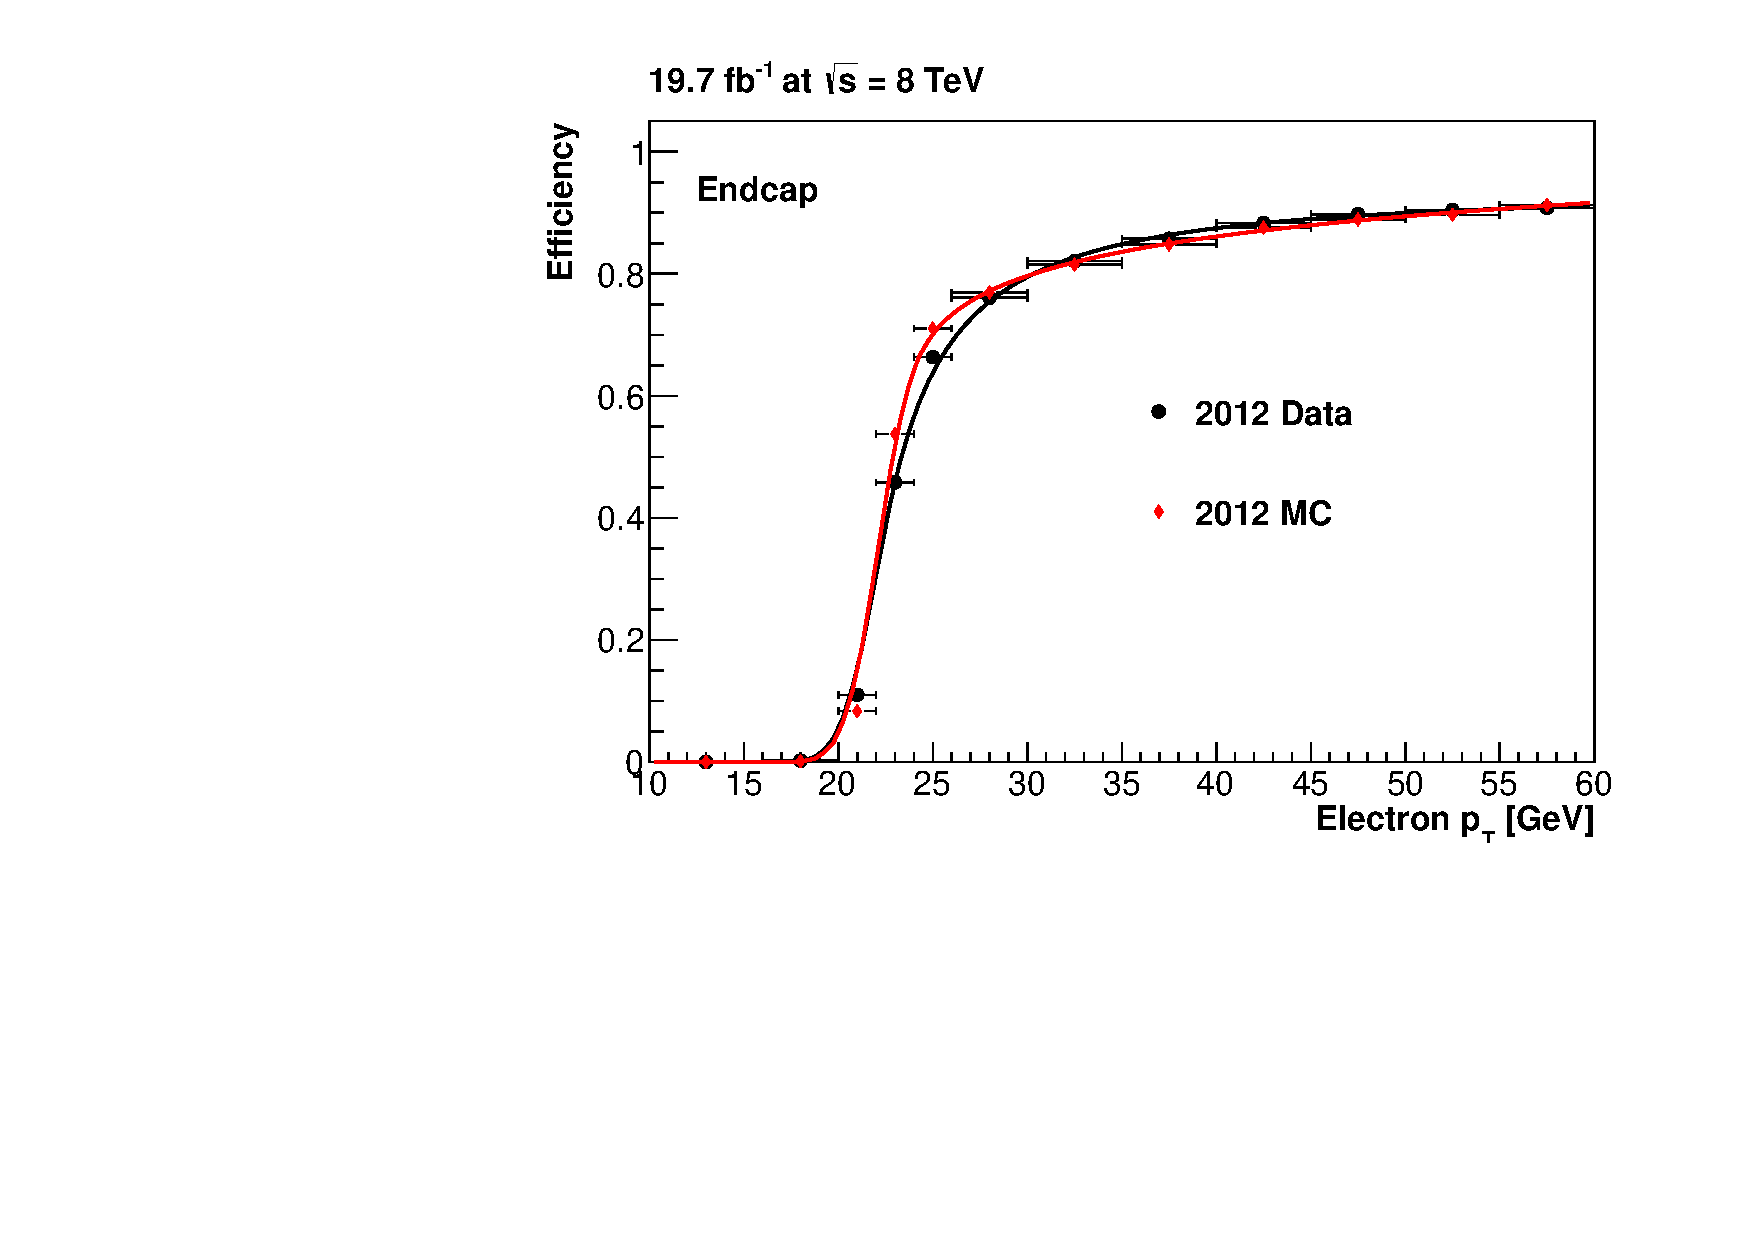
\includegraphics[width=0.5\textwidth]{plots/TagAndProbe/ElectronEndcap2012DatavsMC.pdf}}
\caption{Trigger efficiency as a function of electron $\pt$ measured
in 2012 data and MC in the (left) barrel and (right) endcaps.}
\label{fig:electrontrg}
\end{figure}

\begin{figure}[h!]
\subfloat[]{
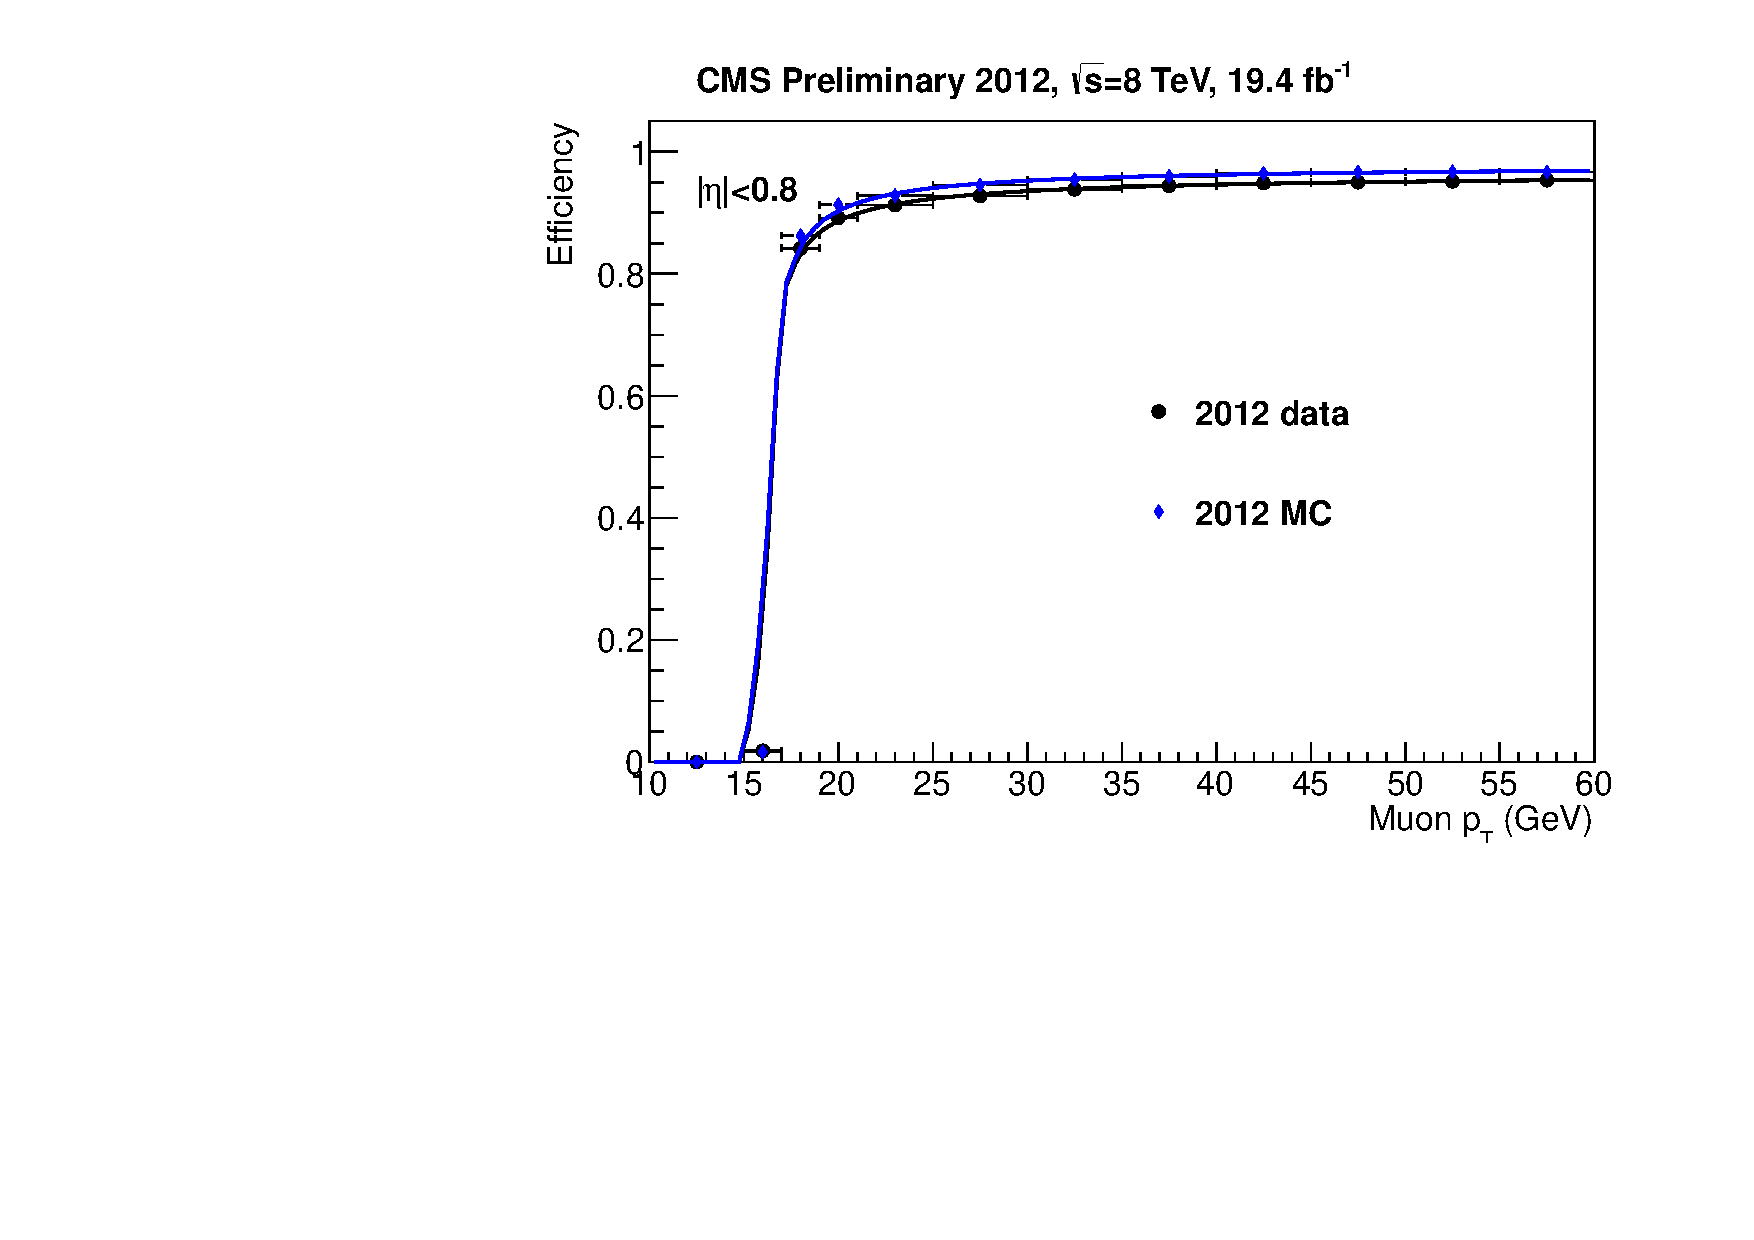
\includegraphics[width=0.5\textwidth]{plots/TagAndProbe/MuonAbsEta082012DatavsMC.pdf}}
\subfloat[]{
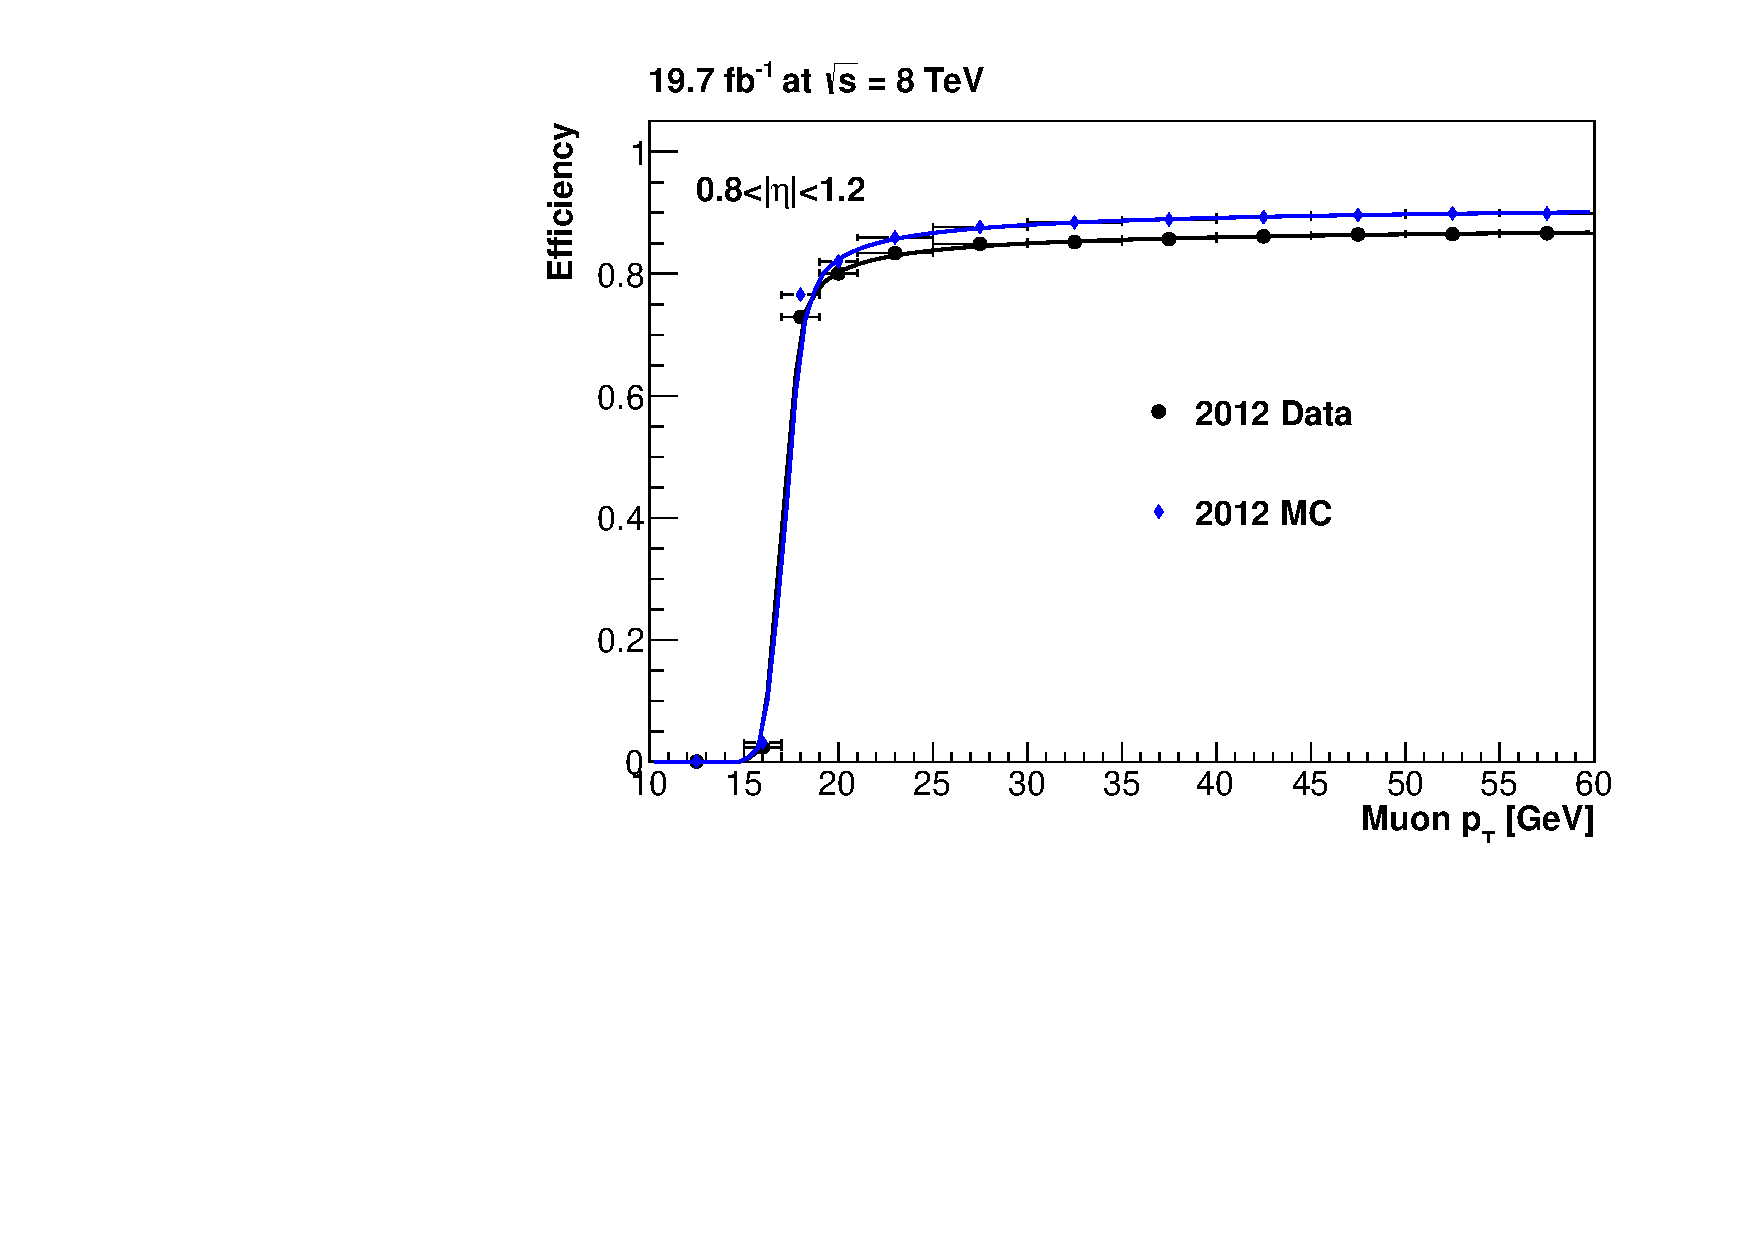
\includegraphics[width=0.5\textwidth]{plots/TagAndProbe/MuonAbsEta122012DatavsMC.pdf}}

\begin{center}
\subfloat[]{
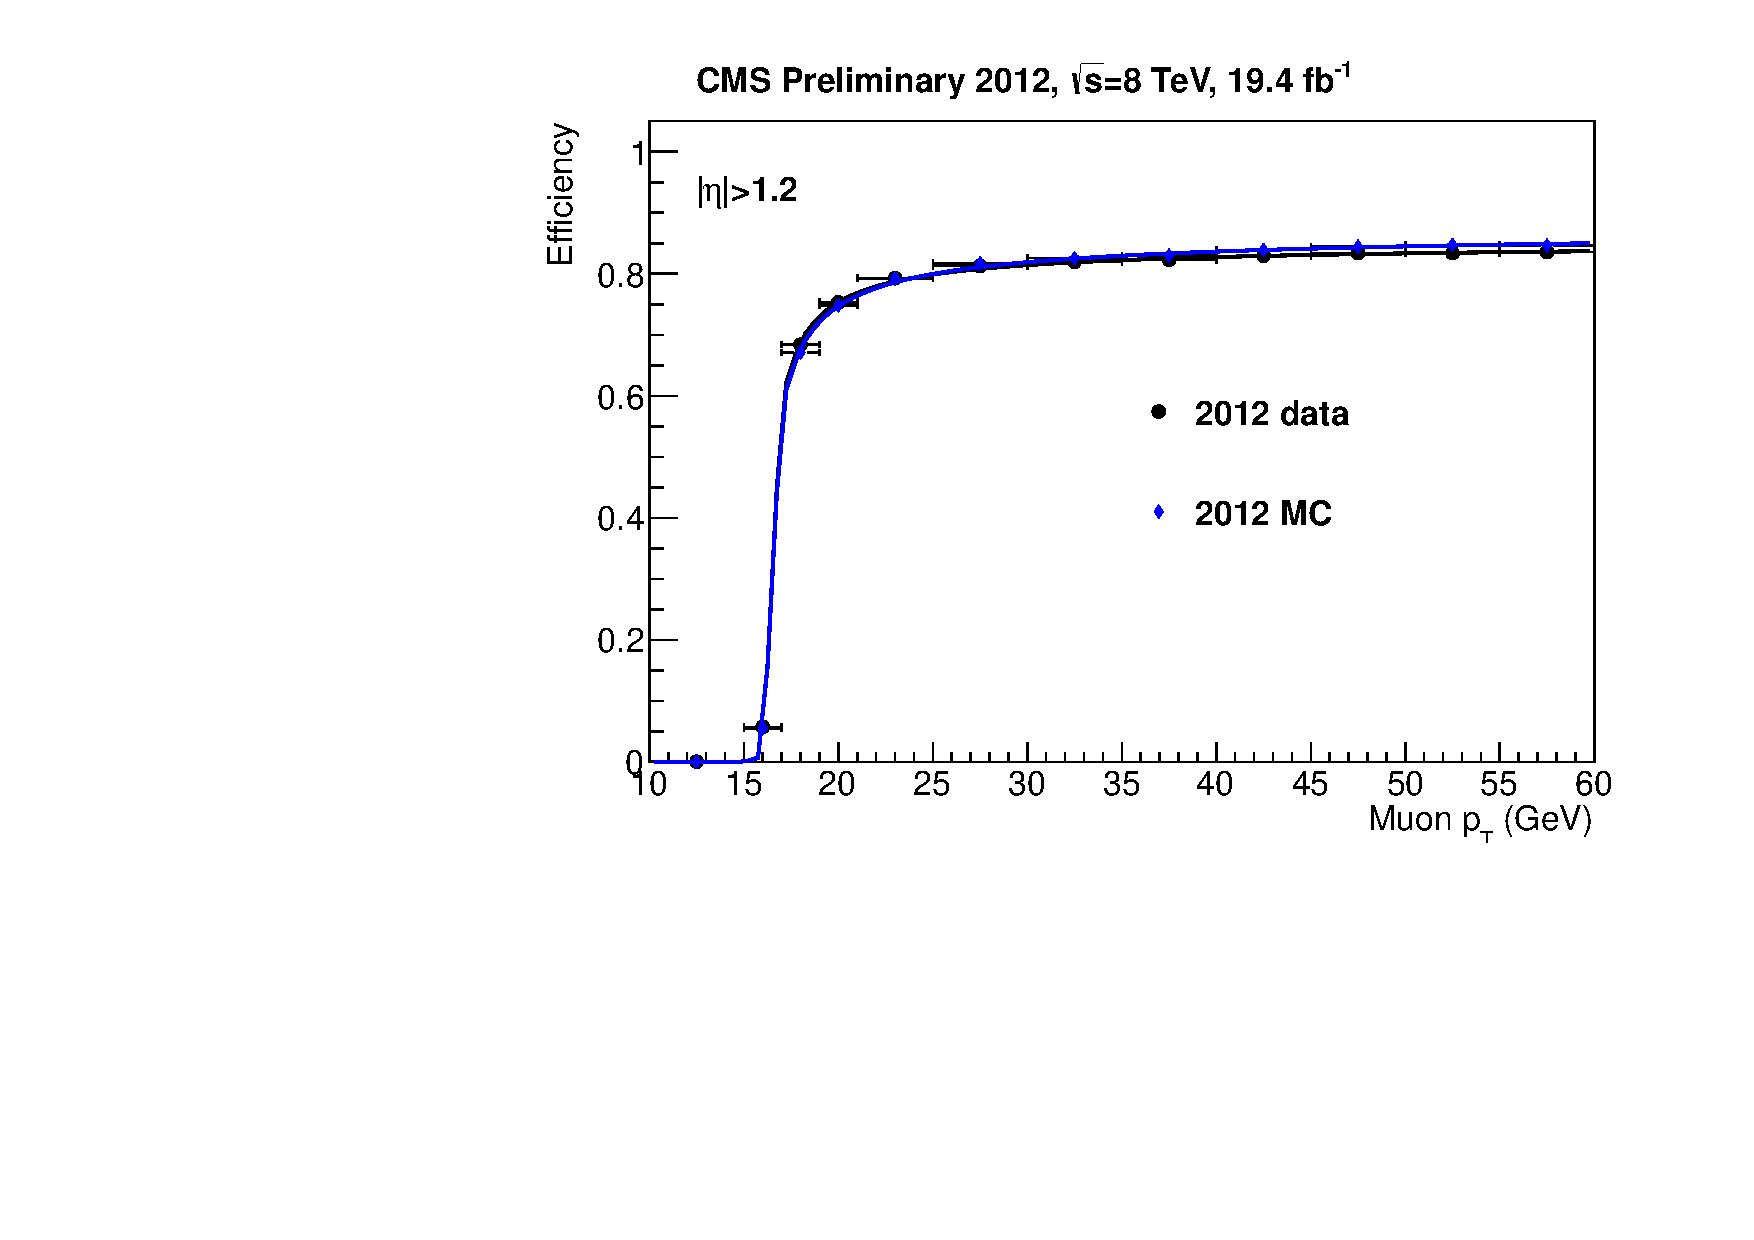
\includegraphics[width=0.5\textwidth]{plots/TagAndProbe/MuonAbsEndcap2012DatavsMC.pdf}}
\end{center}
\caption{Trigger efficiency as a function of muon $\pt$ measured in
2012 data and MC in the region (top left) $|\eta|$ $<$ 0.8, (top right) 0.8
$<$ $|\eta|$ $<$ 1.2 and (bottom) $|\eta|$ $>$ 1.2.}
\label{fig:muontrg}
\end{figure}

\section{Systematics}
\label{sec:systematics}

The systematic uncertainties consist of two different types:

\begin{itemize} 
\item Normalisation uncertainties: these affect the yield of a particular background or
signal.
\item Shape uncertainties: these affect the shape of the signal or background, or in
other words the number of signal or background events in a particular bin rather
than the overall number.
\end{itemize}

The way in which these different types of uncertainties are incorporated in the
final results is described in section \ref{sec:signalextraction}. The different
sources of uncertainties and their chosen values is described in the next
section separately for the normalisation and shape uncertainties.

\subsection{Normalisation Uncertainties}
\label{sec:systematicUncertainties_yield}

The uncertainties in the analysis which contribute to the normalisation of the
background or signal processes are as follows:

\begin{itemize}
\item \textbf{ID, isolation and trigger efficiencies for the electrons, muons and
hadronic taus}.\\
Data to MC scale factors as described in \cite{CMS_AN_2013-171}
are measured for this analysis and applied to correct for differences in these
efficiencies in MC compared with data. The estimated uncertainty in these
measurements are combined in quadrature. For the electrons and muons, this
amounts to a 2$\%$ normalisation uncertainty, which is applied to all
backgrounds in which the yield is taken from MC and signal.
For the hadronic taus a 6$\%$ uncertainty
is measured on the tau identification efficiency using 
$Z/\gamma^{*} \to \tau\tau \to \mu\tau_{had}$
events~\cite{TauIDRecommendation}. For the hadronic tau leg of the trigger, the
uncertainty is 3.0$\%$ for the triggers of the $e\tau_{had}$ and $\mu\tau_{had}$
channels and 4.5$\%$ for each leg of the trigger in the $\tau_{had}\tau_{had}$
channels. These uncertainties are applied to all backgrounds in which the yield
is taken from MC and signal.
\item \textbf{$e \to \tau_{had}$ and $\mu \to \tau_{had}$ fake--rates} \\
The uncertainty on the $e \to \tau_{had}$ fakerate is determined as part of
its measurement, and a description can be found in \cite{CMS_AN_2013-171}.
This amounts to an uncertainty of $30\%$, correlated between $\tau_{had}$ candidates
reconstructed in any tau decay mode. The uncertainty on the rate of $\mu \to \tau_{had}$
fakes is taken from the Tau POG~\cite{TauIDRecommendation}, amounting to $30\%$. 
\item \textbf{b--tag scale--factors} \\
Uncertainties on b--tagging efficiencies and mistag rates as function of jet
$P_{T}$ and $\eta$ for a particular b-tag working point of the CSV discriminator
(in the case of this analysis the medium working point) are provided by the BTV 
POG~\cite{BTagSFRecommendation}. The effect of these uncertainties on the
analysis is evaluated by varying the scale factors applied within their
recommended uncertiainties and evaluating the overall change in yield as a
result in each channel and category for each background. For those backgrounds
with a non-negligible variation as a result of this uncertainty the yield change
is applied as a normalisation uncertainty.
\item \textbf{$Z$--recoil correction} \\
Uncertainties on \MET resolution and response are accounted for
by varying the $Z$--recoil correction parameters within the uncertainties determined within the method.
\MET and all \MET related observables (including $M_{\tau\tau}$) are recomputed after each such variation.
\item \textbf{Background Normalisation} \\
The normalisation uncertainties on the backgrounds are evaluated where possible
by using alternative methods for estimation and studying the difference in yield,
and/or an uncertainty is applied which covers the statistical uncertainty on the
yield prediction from the default method. 

The normalization of the $Z/\gamma^{*} \to \tau\tau$ embedded samples in the inclusive event
category, obtained using Monte Carlo samples as described in
section~\ref{sec:backgroundEstimation_Ztautau}, is attributed an uncertainty of
$3\%$. The uncertainty as a result of extrapolation from the inclusive selection
to the category selection is 5$\%$ in the 2jet--0tag and 2jet--1tag categories,
and 6$\%$ in the 2jet--2tag category. An additional uncertainty on the $Z/\gamma^{*} \to \tau\tau$ 
is included to account for the subtraction of
the $t \bar{t}$ contamination in the embedded samples, where the size of the
uncertainty is equal to the size of the contamination. 

The $Z/\gamma^{*} \to \ell\ell$ ($\ell = e$, $\mu$) background is very small
after the requirement of 2 jets, and so the dominant uncertainty is from the
statistical uncertainty on the yield estimate. This uncertainty is estimated separately
for the components where it is either a jet or a lepton which fakes the hadronic 
tau. The uncertainty on the jet component is 20$\%$ (20$\%$) in the 2jet--0tag,
20$\%$ (25$\%$) int the 2jet--1tag and 90$\%$ (70$\%$) in the 2jet--2tag
category in the $\mu\tau_{had}$ and $e\tau_{had}$ channels respectively.
The corresponding uncertainties on the leptonic component
are 30$\%$ (20$\%$) in 2jet--0tag, 60$\%$ (20$\%$) in 2jet--1tag and 60$\%$
(40$\%$) in 2jet--2tag. 

The uncertainty on the $t \bar{t}$ cross-section amounts to $10\%$, and on the single top and di--boson
production cross--sections amounts to $15\%$.

The normalization of the $W$ + jets background is obtained from data, 
using the high $M_{T}$ sideband extrapolation method described in
section~\ref{sec:backgroundEstimation_WplusJets}. The uncertainty on the W
estimate is dominated by the data statistics available in this control region, and
amounts to 10$\%$ in the 2jet--0tag category, 40$\%$ in the 2jet--1tag category
and 100$\%$ in the 2jet-2tag category. 

The uncertainty on the normalization of QCD background is obtained by adding the
statistical uncertainty on the yield of events selected in the QCD dominated control regions
described in section~\ref{sec:backgroundEstimation_QCD} in quadrature with the
uncertainty on opposite sign - same sign factor of 1.06, which is around 10$\%$. 

%\item \textbf{Theoretical Uncertainties} \\
\item \textbf{Luminosity} \\
  The uncertainty on the luminosity amounts to $2.6\%$ for $2012$ data.
  This uncertainty is applied to the signal
  and to $Z/\gamma^{*} \to \ell\ell$ ($\ell = e$, $\mu$), $Z/\gamma^{*} \to
  \tau\tau$, $t \bar{t}$, single top and di--boson backgrounds. 
  The normalization of the $W$ + jets and QCD backgrounds is obtained from data and hence not subject to the luminosity uncertainty.
\end{itemize}

\subsection{Shape Uncertainties}
\label{sec:systematicUncertainties_yield}

\begin{itemize}

\item \textbf{$\tau_{had}$ energy scale} \\
When studying mass distributions, the shape of the distribution is directly
dependent on the energy scale of the objects making up the mass. Thus the
$m_{\tau\tau}$ and 4 body mass shapes are sensitive to the tau energy scale.
To incorporate this uncertainty, the energy scale of hadronically decaying taus is varied by $3\%$,
following the recommendation of the Tau POG~\cite{TauIDRecommendation}. 
in the previous section.
\item \textbf{$Z \to \ell\ell$ lepton energy scale}\\
A shape uncertainty is also added for the $Z \to \ell\ell$ contribution for the
events in the $e\tau_{had}$ and $\mu\tau_{had}$ channels where a lepton fakes a
hadronic tau, to account for the effect of the energy scale of the lepton fake.
This energy scale mismeasurement is estimated to give a shift of up to 2$\%$ in the
mass shape of the contribution, and hence a shape systematic amounting to the
2$\%$ shift up and down is included to cover for this effect.

\end{itemize}

\section{Results}
\label{sec:results}

\subsection{Signal Extraction}
\label{sec:signalextraction}

\subsection{Limit and Significance}
\label{sec:significance}

\begin{figure}[h!]
\subfloat[]{
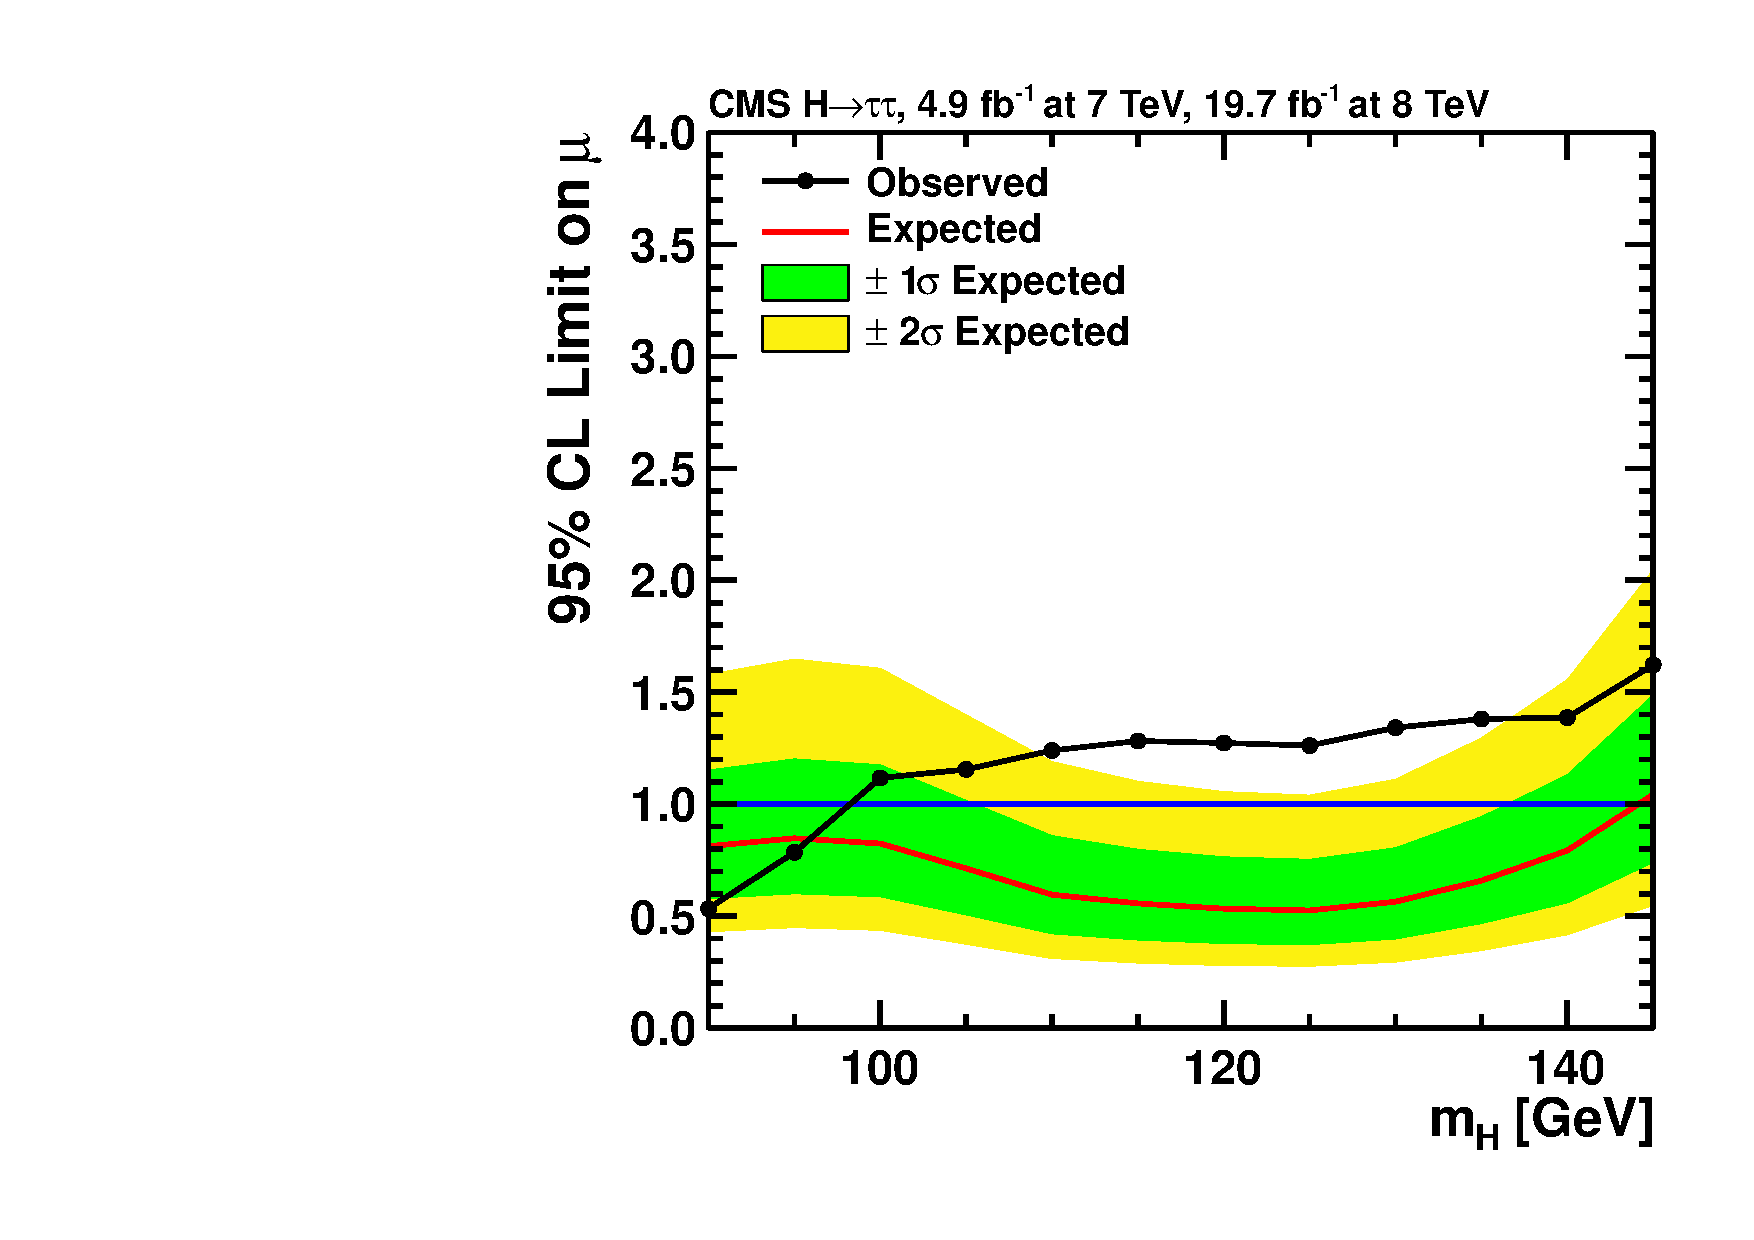
\includegraphics[width=0.5\textwidth]{plots/htt-sm/cmb_limit.pdf}}
\subfloat[]{
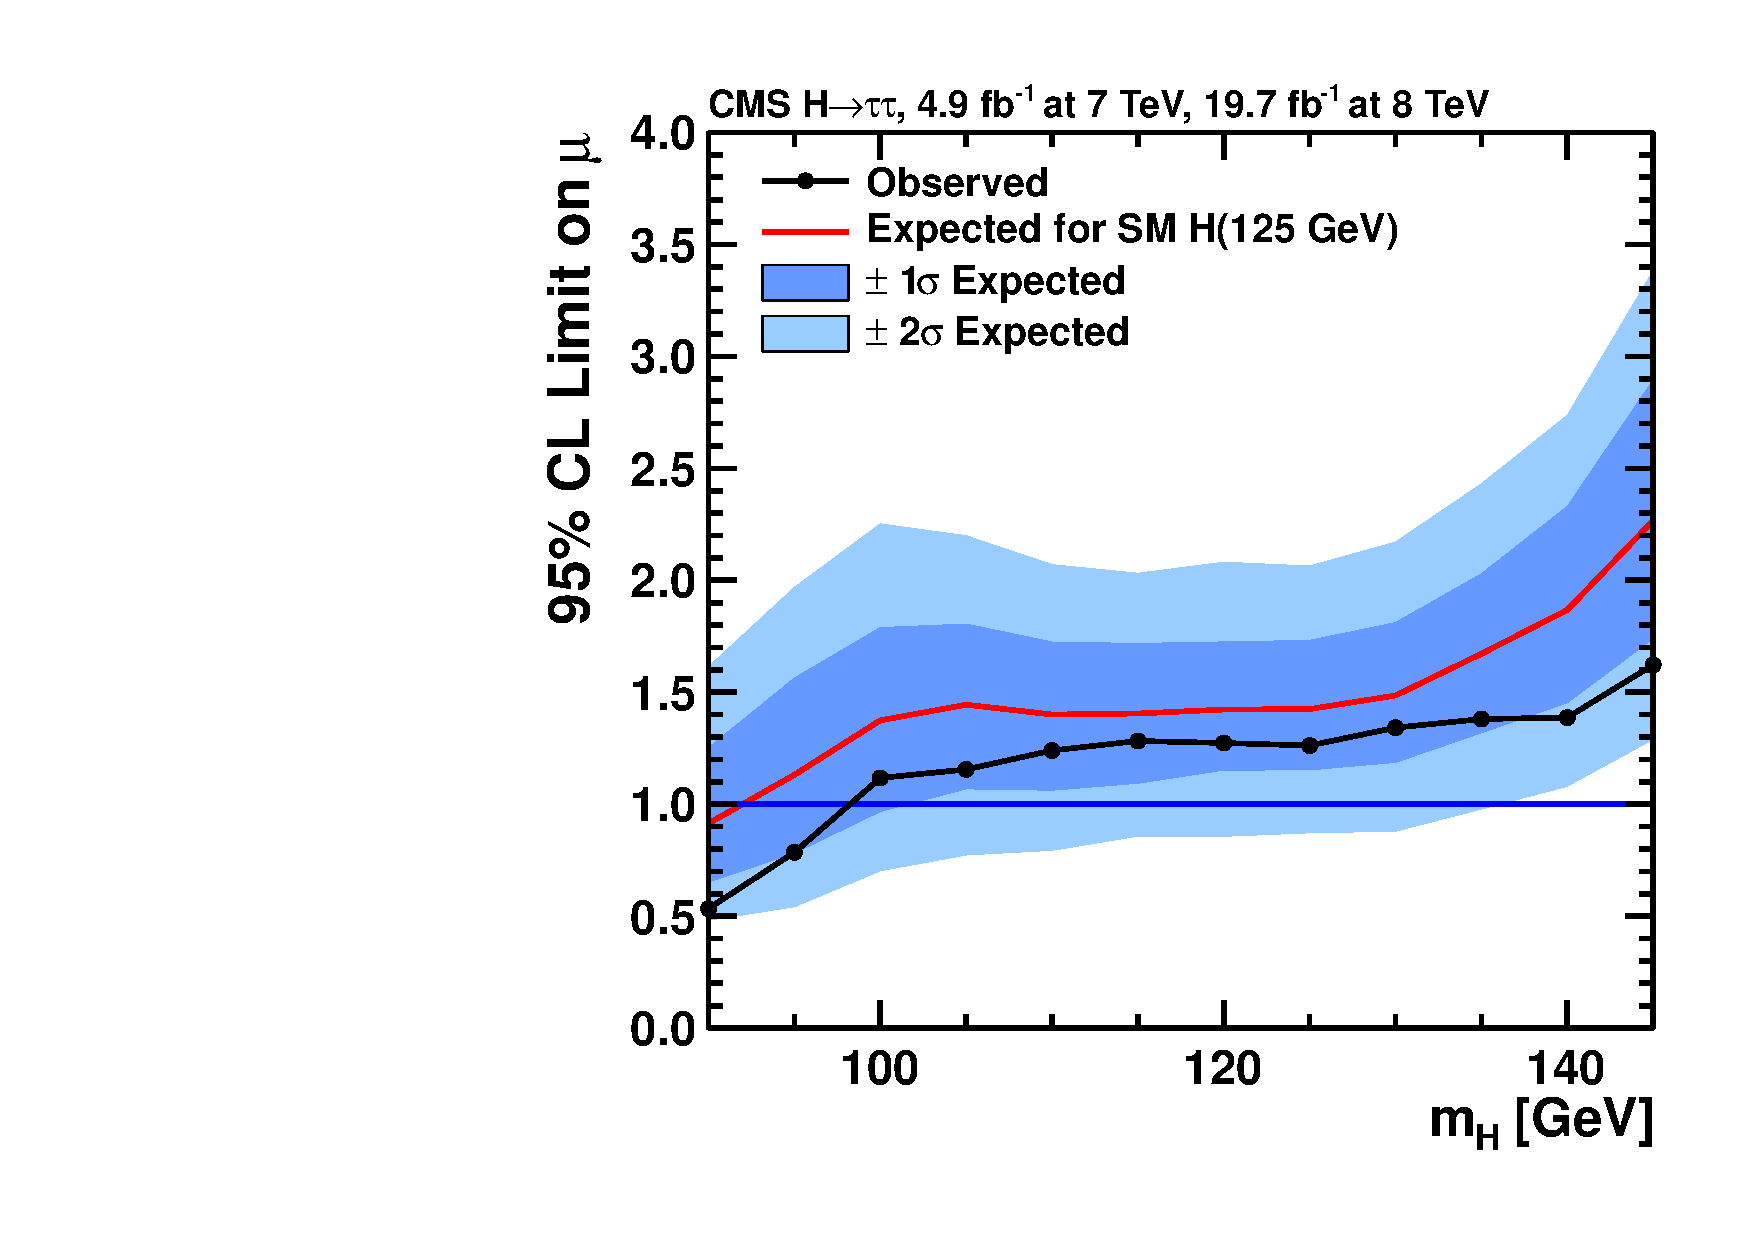
\includegraphics[width=0.5\textwidth]{plots/htt-sm/cmb_limit_signalinjected.pdf}}
\caption{Expected and observed limit}
\label{fig:results-limit}
\end{figure}

\begin{figure}[h!]
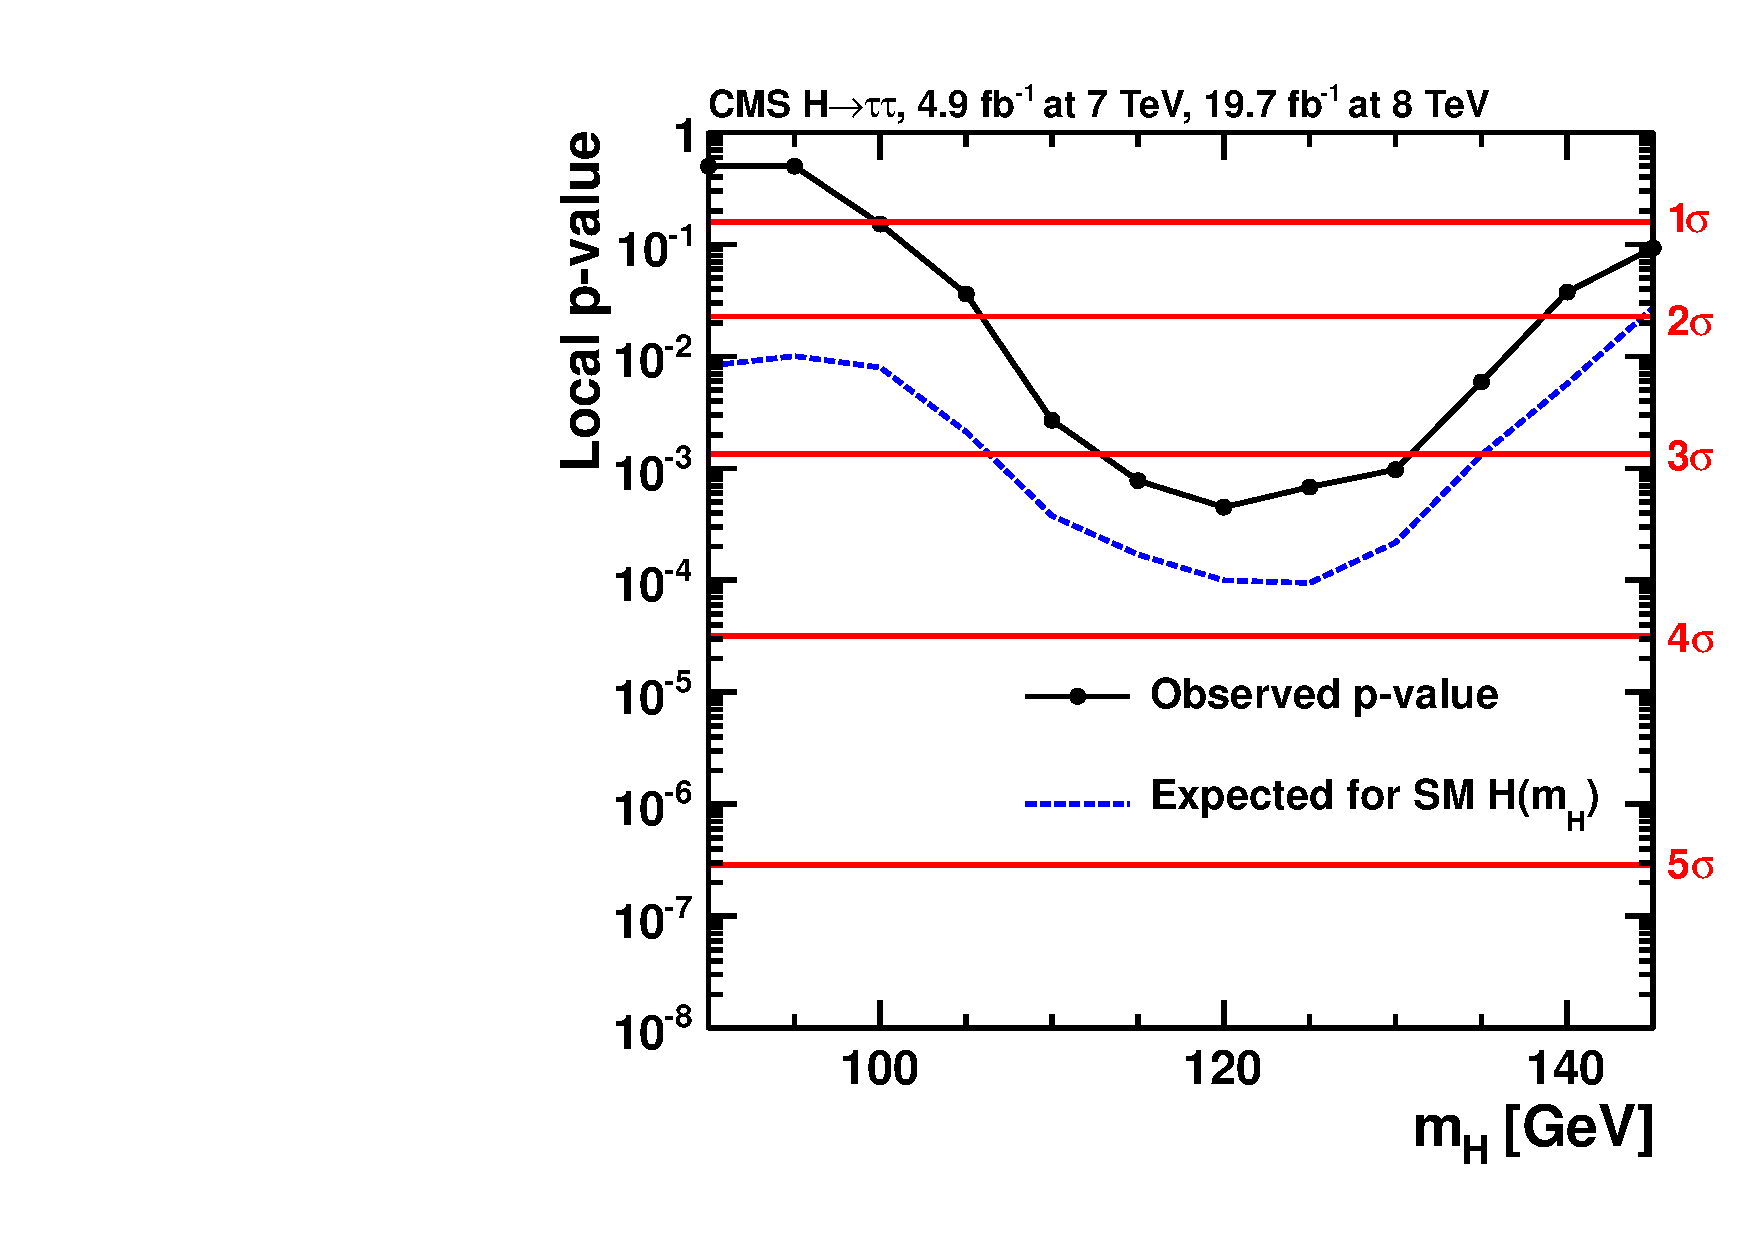
\includegraphics[width=0.5\textwidth]{plots/htt-sm/cmb_p-value.pdf}
\caption{P value}
\label{fig:results-limit}
\end{figure}


\subsection{Consistency with $125~\GeV$ Higgs}
\label{sec:consistency}

\begin{figure}[h!]
\subfloat[]{
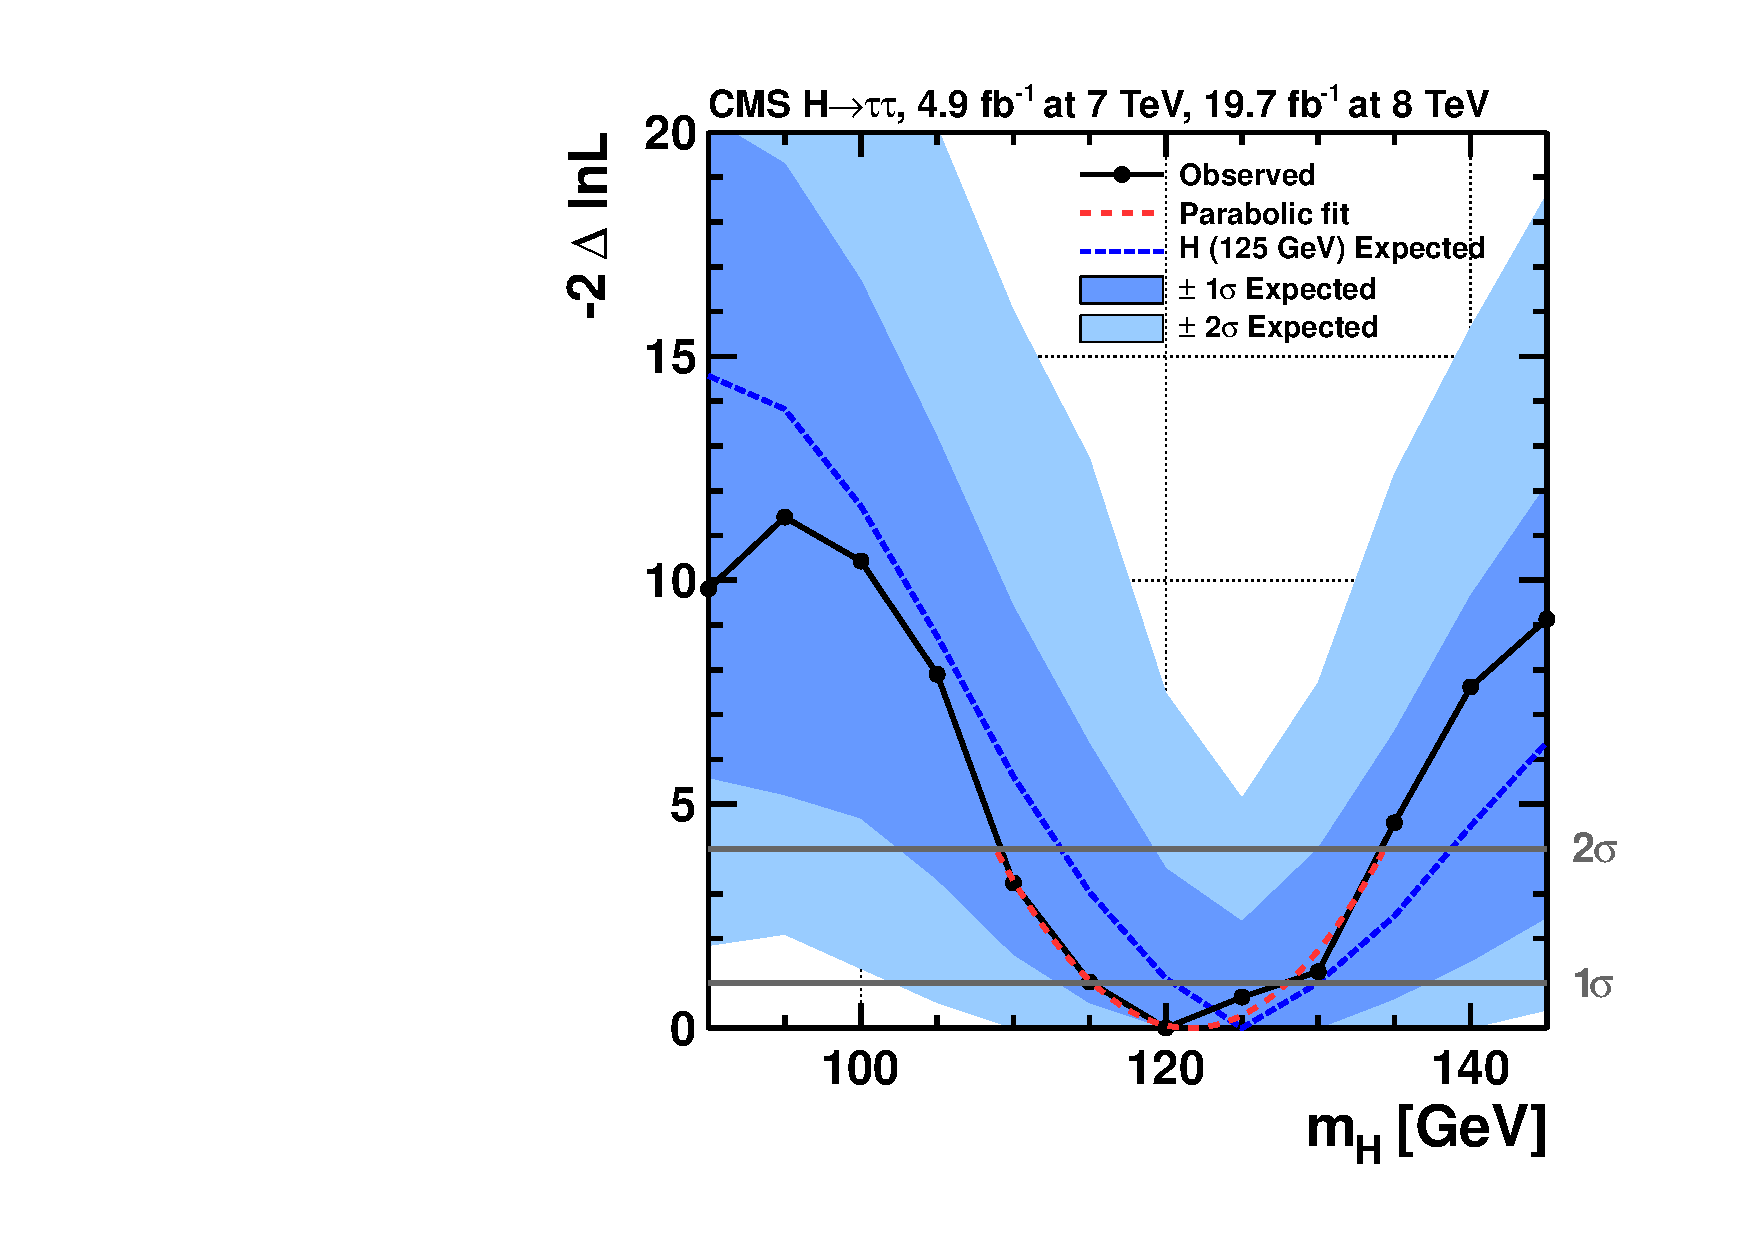
\includegraphics[width=0.5\textwidth]{plots/htt-sm/cmb-mass_scan.pdf}}
\subfloat[]{
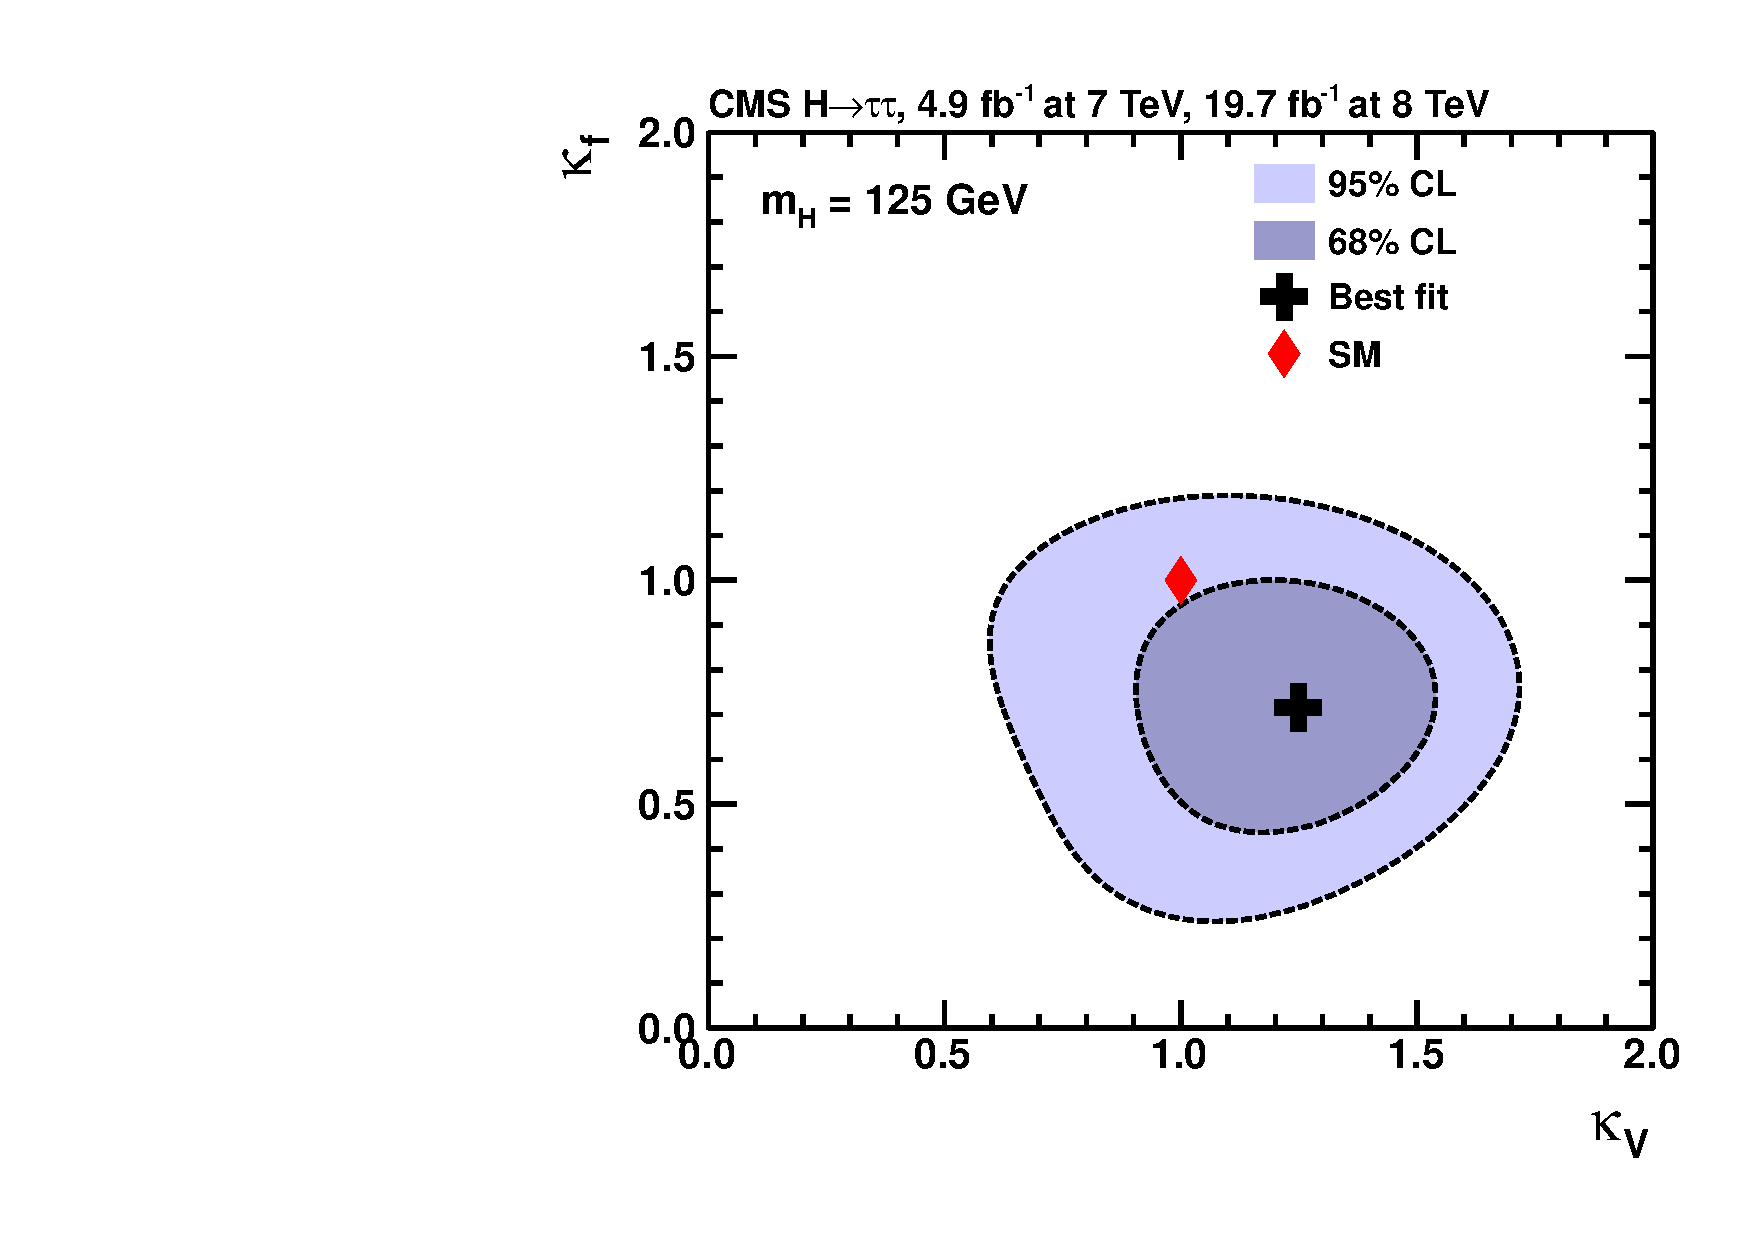
\includegraphics[width=0.5\textwidth]{plots/htt-sm/cmb-scan-hww-CV-CF-125.pdf}}
\caption{Mass scan and couplings}
\label{fig:results-properties}
\end{figure}

